\defChapterTarget{Scenari}

    \section{Scenario 1}
    Mario è uno studente al primo anno di liceo scientifico che a metà del primo
    semestre inizia a mostrare delle lacune in matematica. I genitori sono
    preoccupati del rendimento del figlio e decidono di affidarsi a Ripe4U. I
    genitori accedono dalla homepage alla pagina "I nostri Servizi" cliccando
    sul link con il medesimo nome. Su questa pagina possono filtrare i tipi di
    servizio richiesti, in queIosonosto caso le ripetizioni. La pagina carica le
    ripetizioni per tutte le materie disponibili. In alternativa è possibile
    cercare il serivizio "ripetizioni di matematica" scrivendo nella finestra
    "cerca" "ripetizioni di matematica". Per accedere al servizio "Ripetizioni
    di matematica" è sufficiente un semplice click. I genitori selezionano
    quindi il volontario che dà ripetizioni di matematica, cliccando sopra l'
    immagine. Viene successivamente caricata la pagina con tutte le informazioni
    del volontario inclusi i contatti con cui è possibile fissare un
    appuntamento.
    \begin{figure}[H]
        \centering
        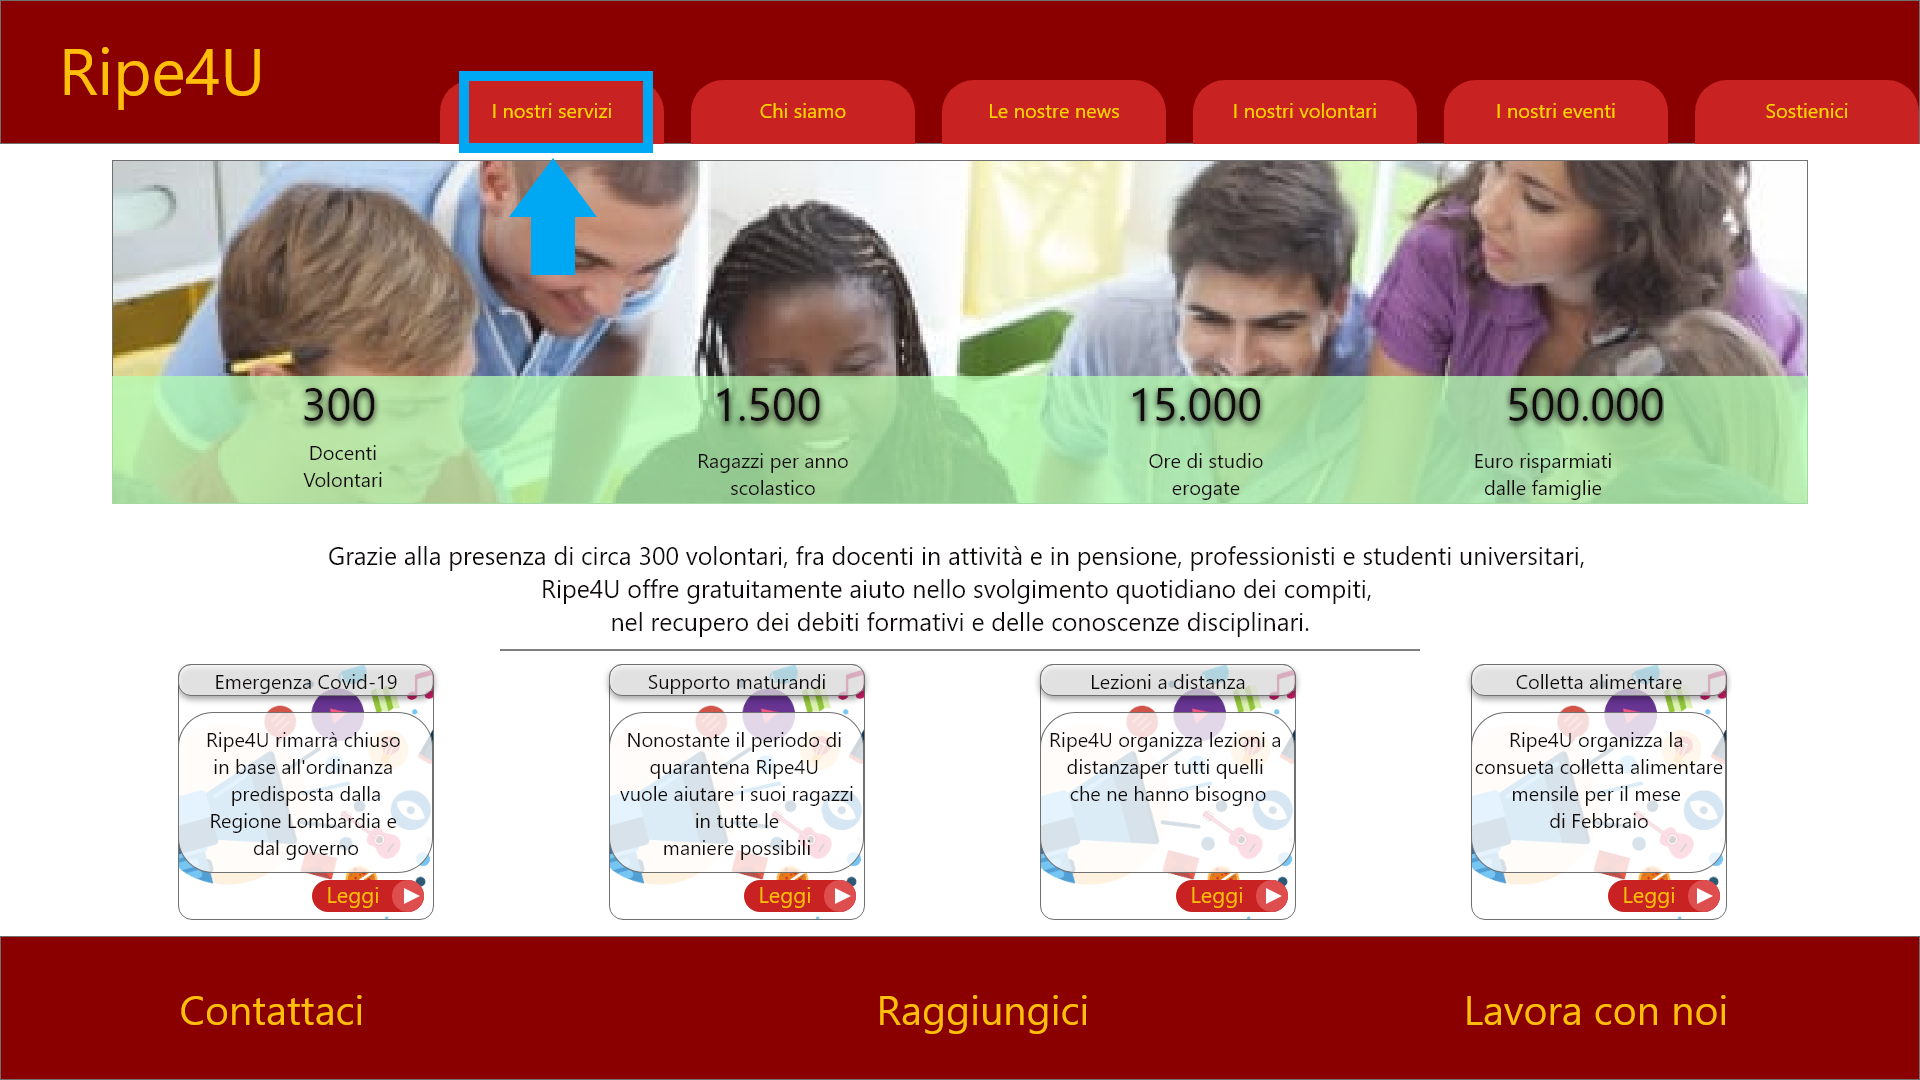
\includegraphics[scale=0.25]{resources/images/scenario1-1.png}
        \caption{I genitori cliccano su "I nostri servizi"}
    \end{figure}
    \begin{figure}[H]
        \centering
        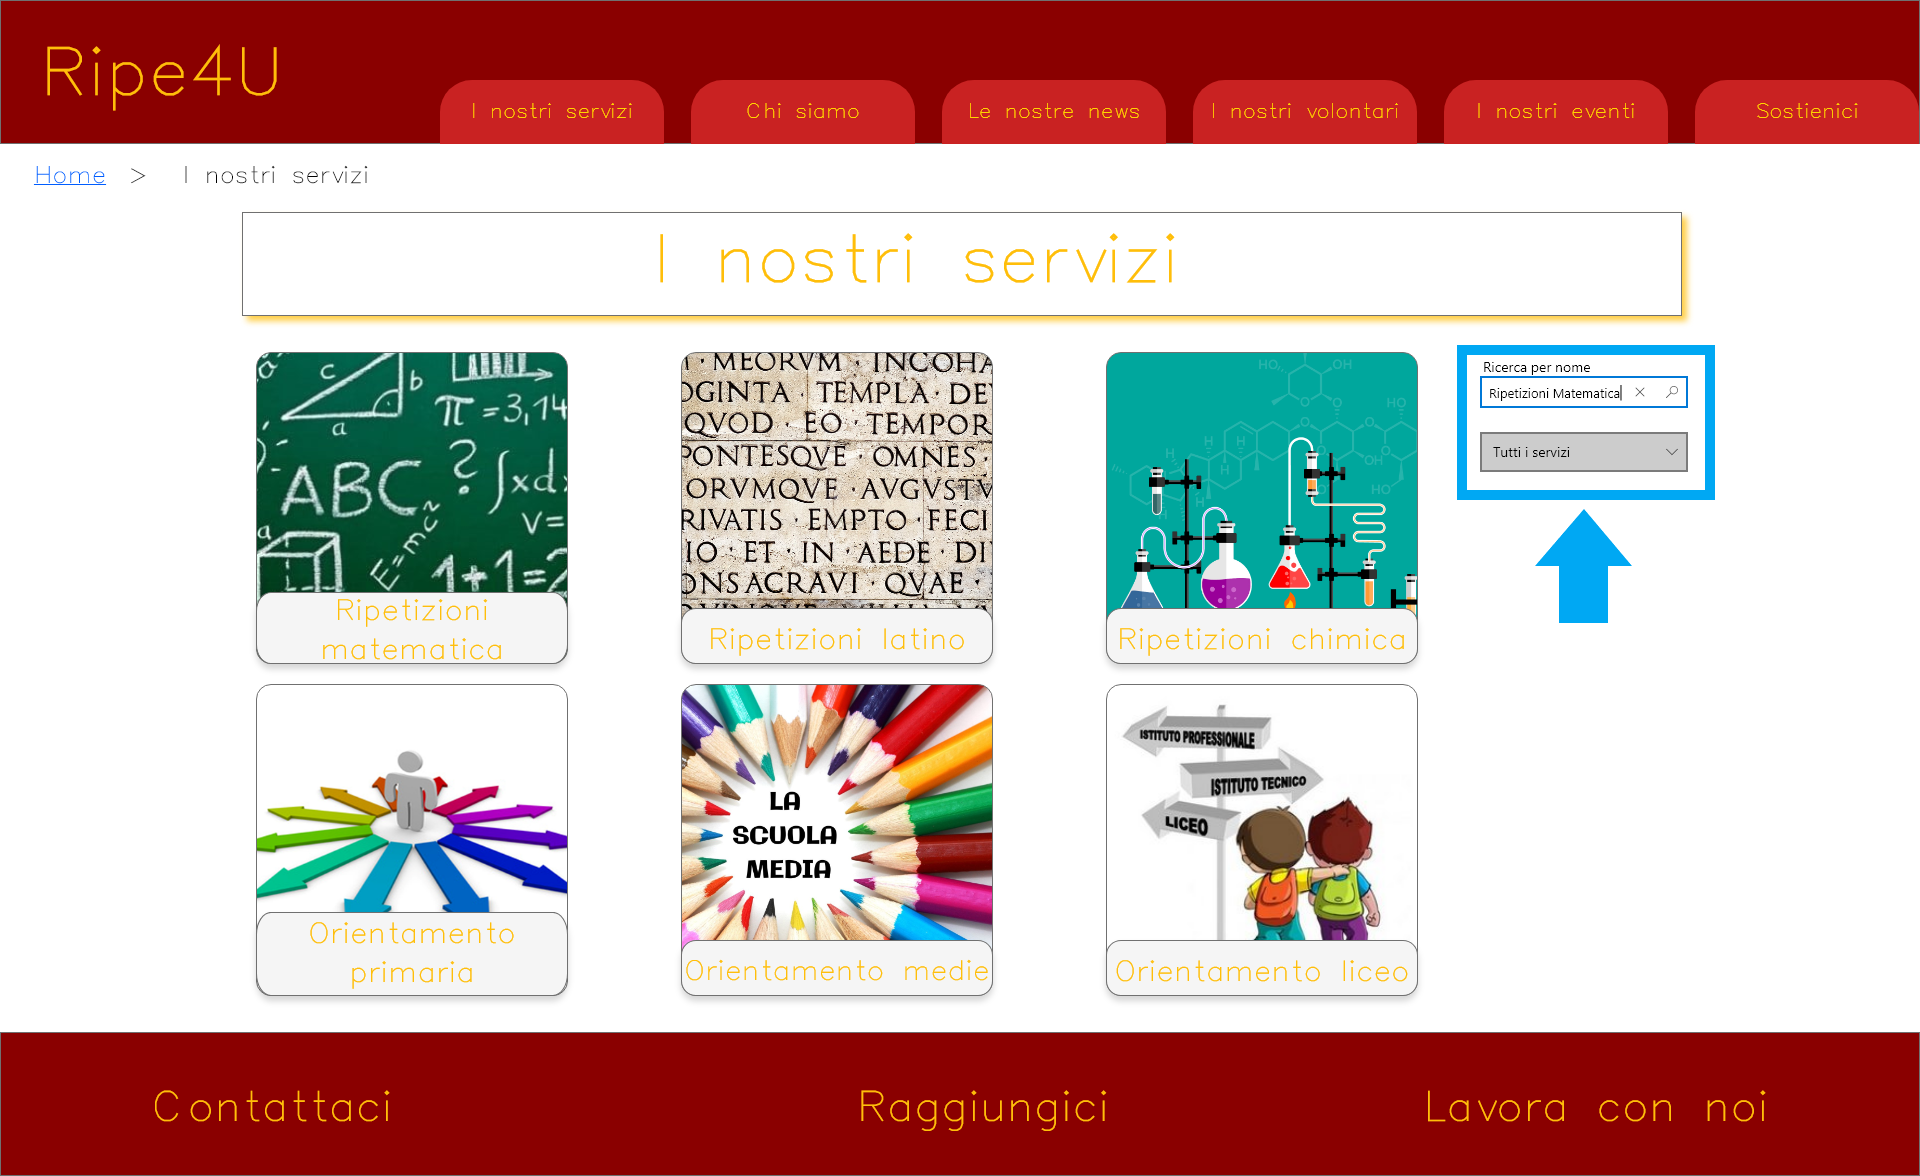
\includegraphics[scale=0.25]{resources/images/scenario1-2.png}
        \caption{I genitori cercano "ripetizioni di matematica"}
    \end{figure}
    \begin{figure}[H]
        \centering
        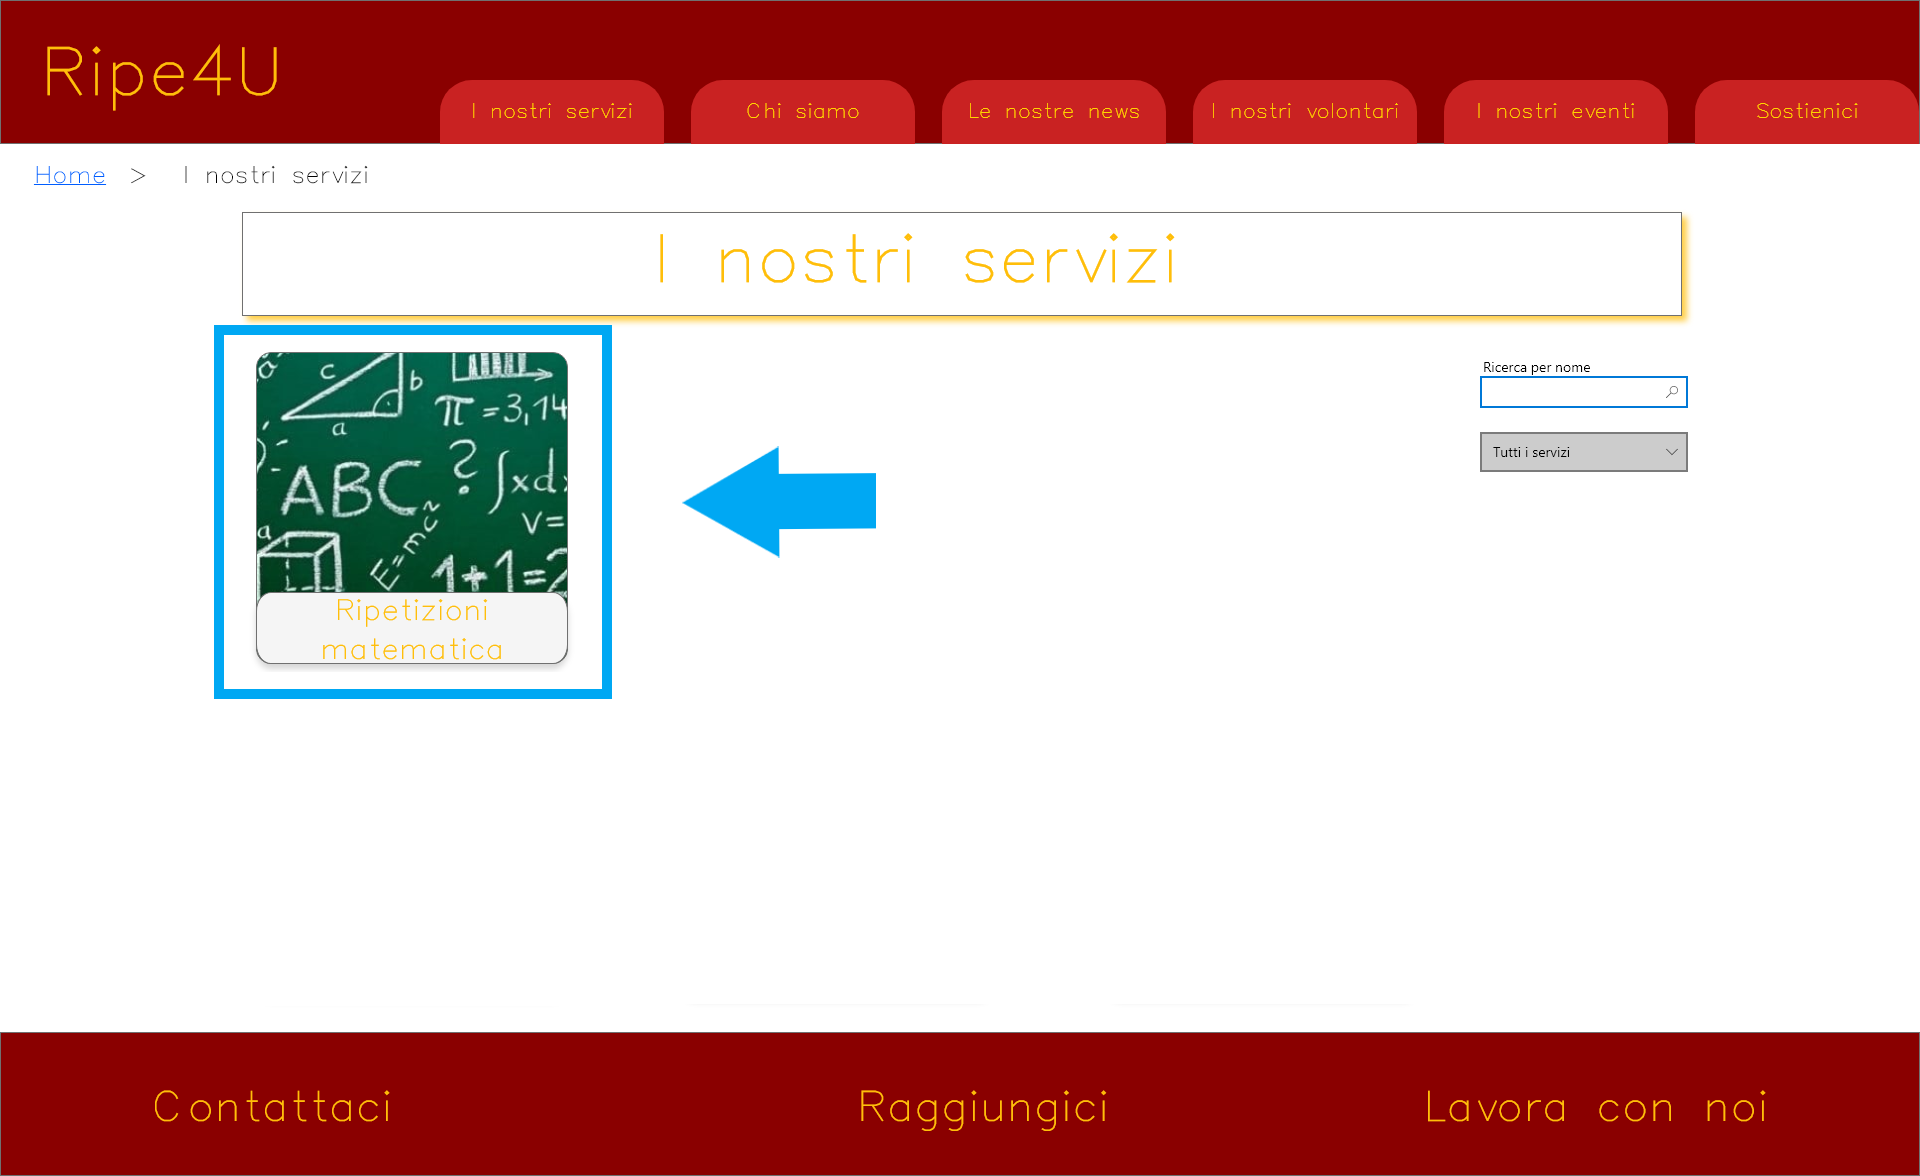
\includegraphics[scale=0.25]{resources/images/scenario1-3.png}
        \caption{I genitori cliccano su "ripetizioni matematica"}
    \end{figure}
    \begin{figure}[H]
        \centering
        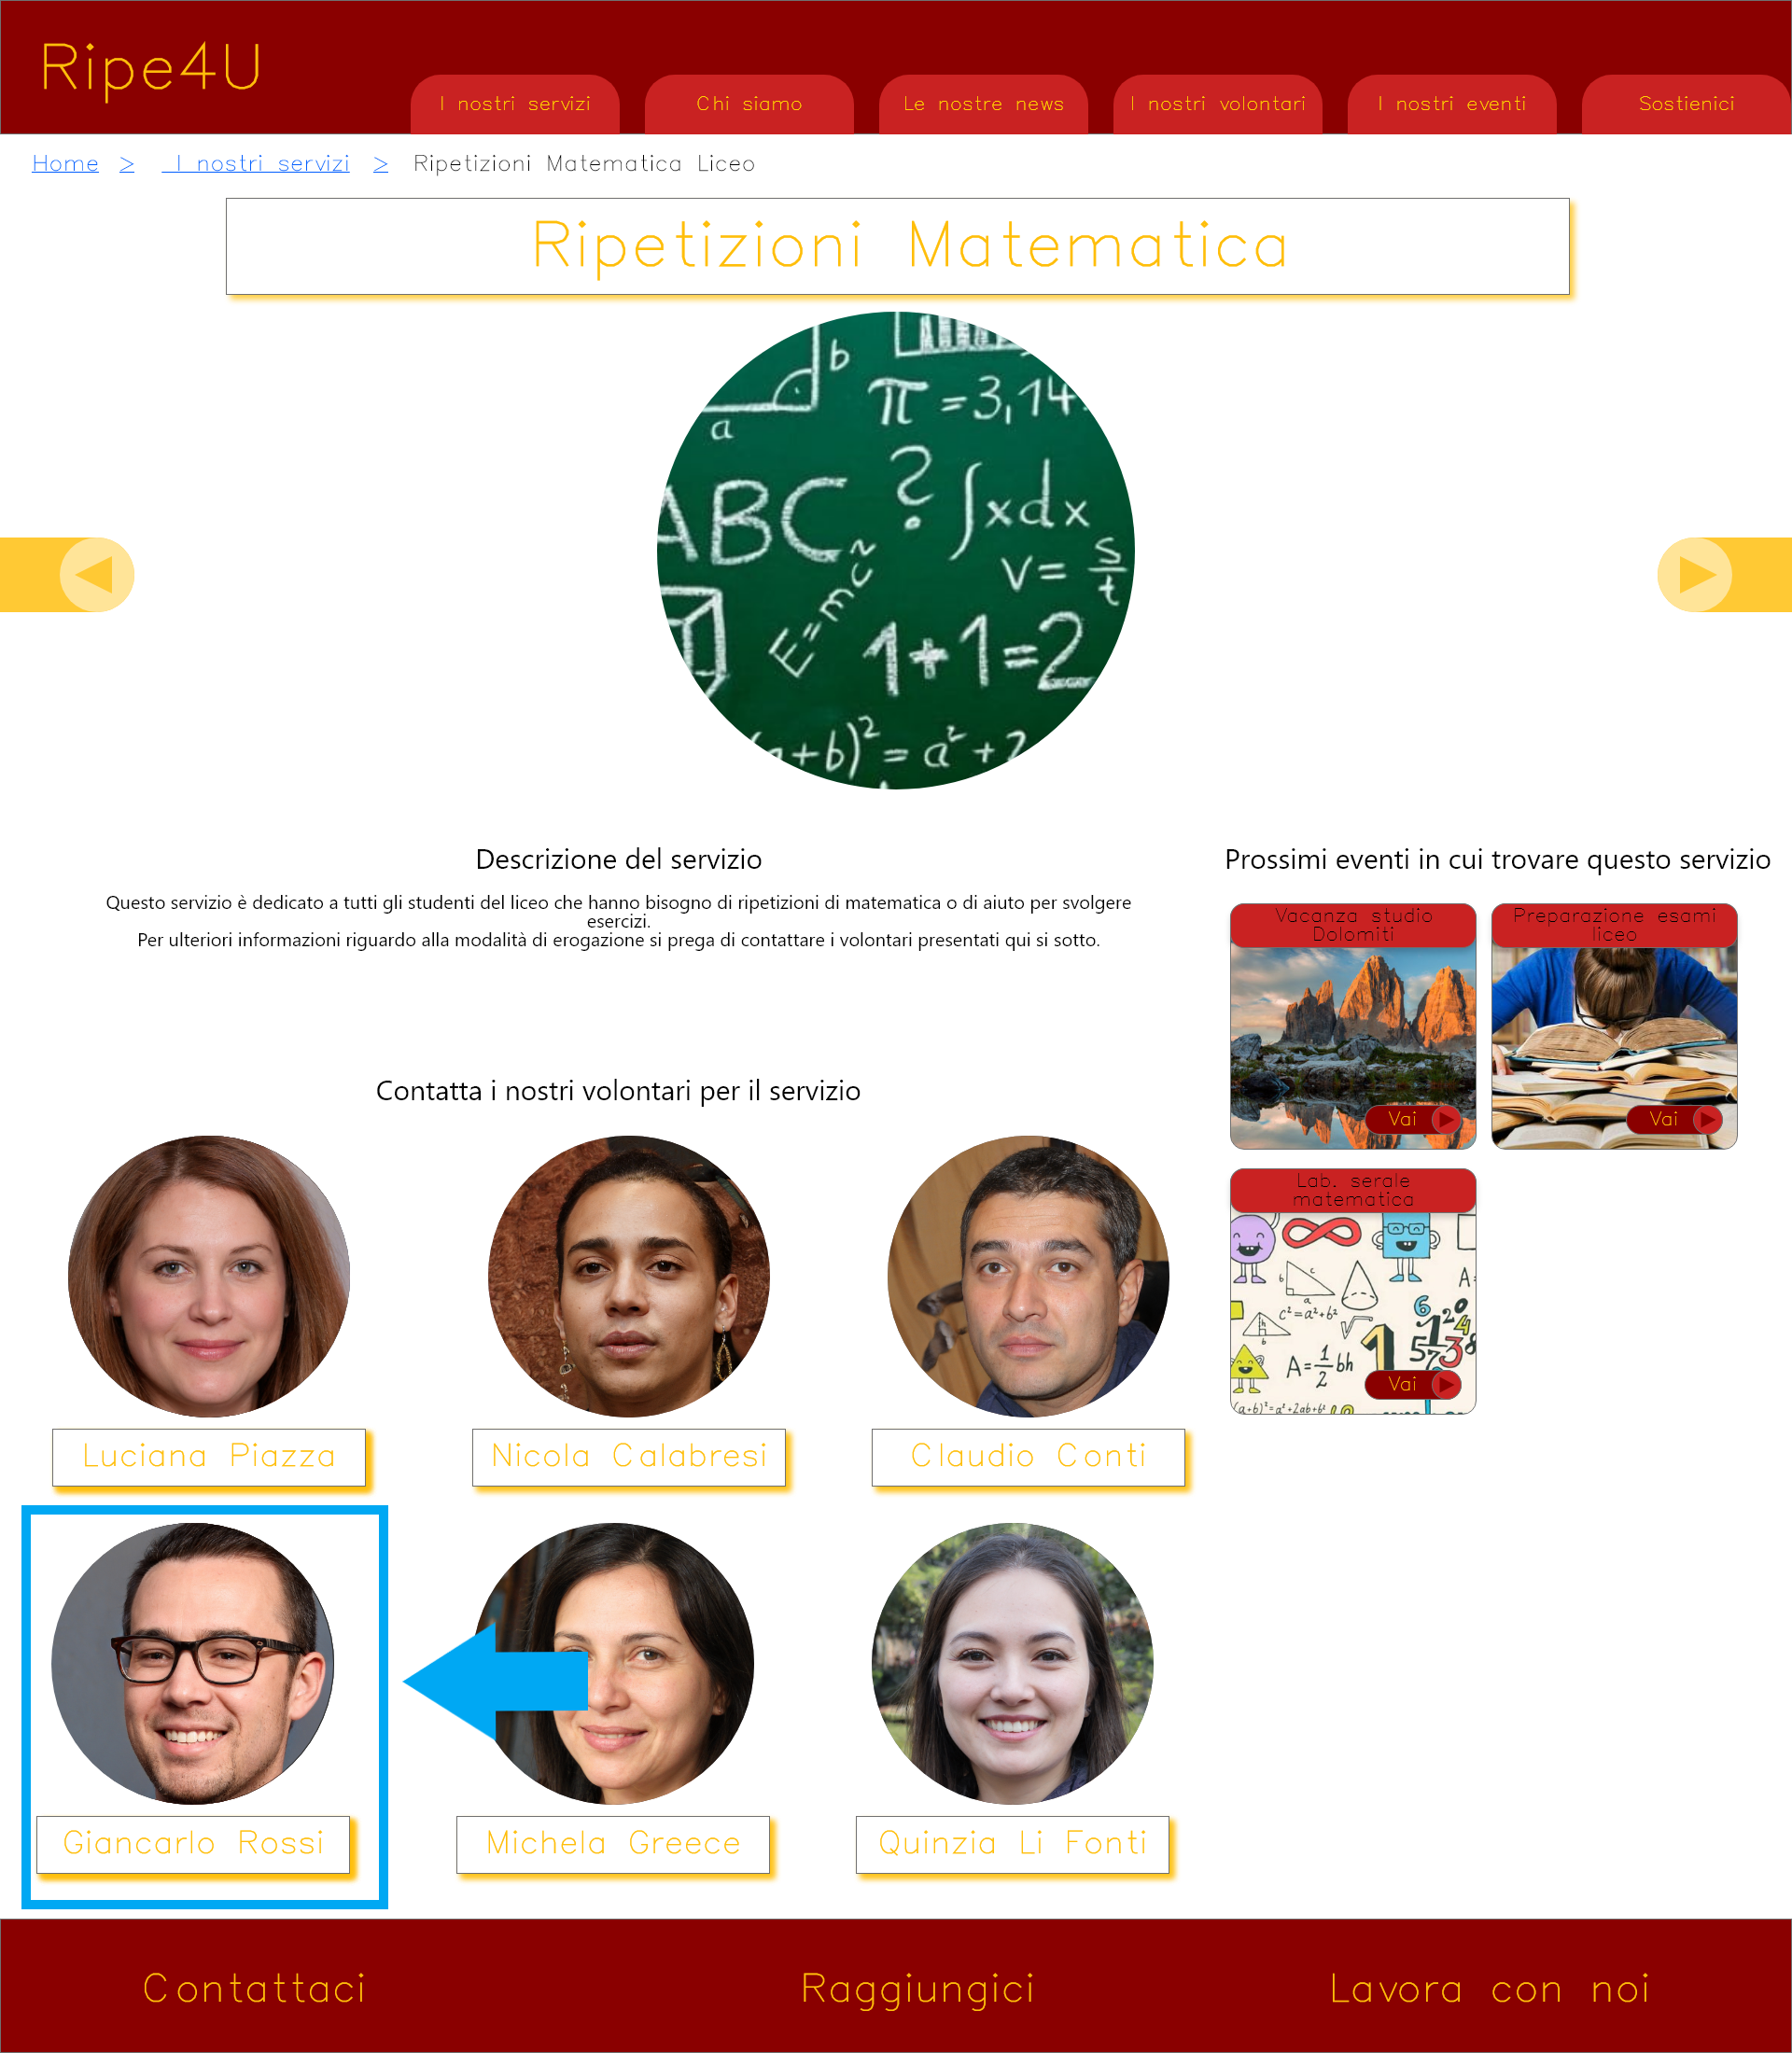
\includegraphics[scale=0.25]{resources/images/scenario1-4.png}
        \caption{I genitori cliccano su "Giancarlo Rossi"}
    \end{figure}
    \begin{figure}[H]
        \centering
        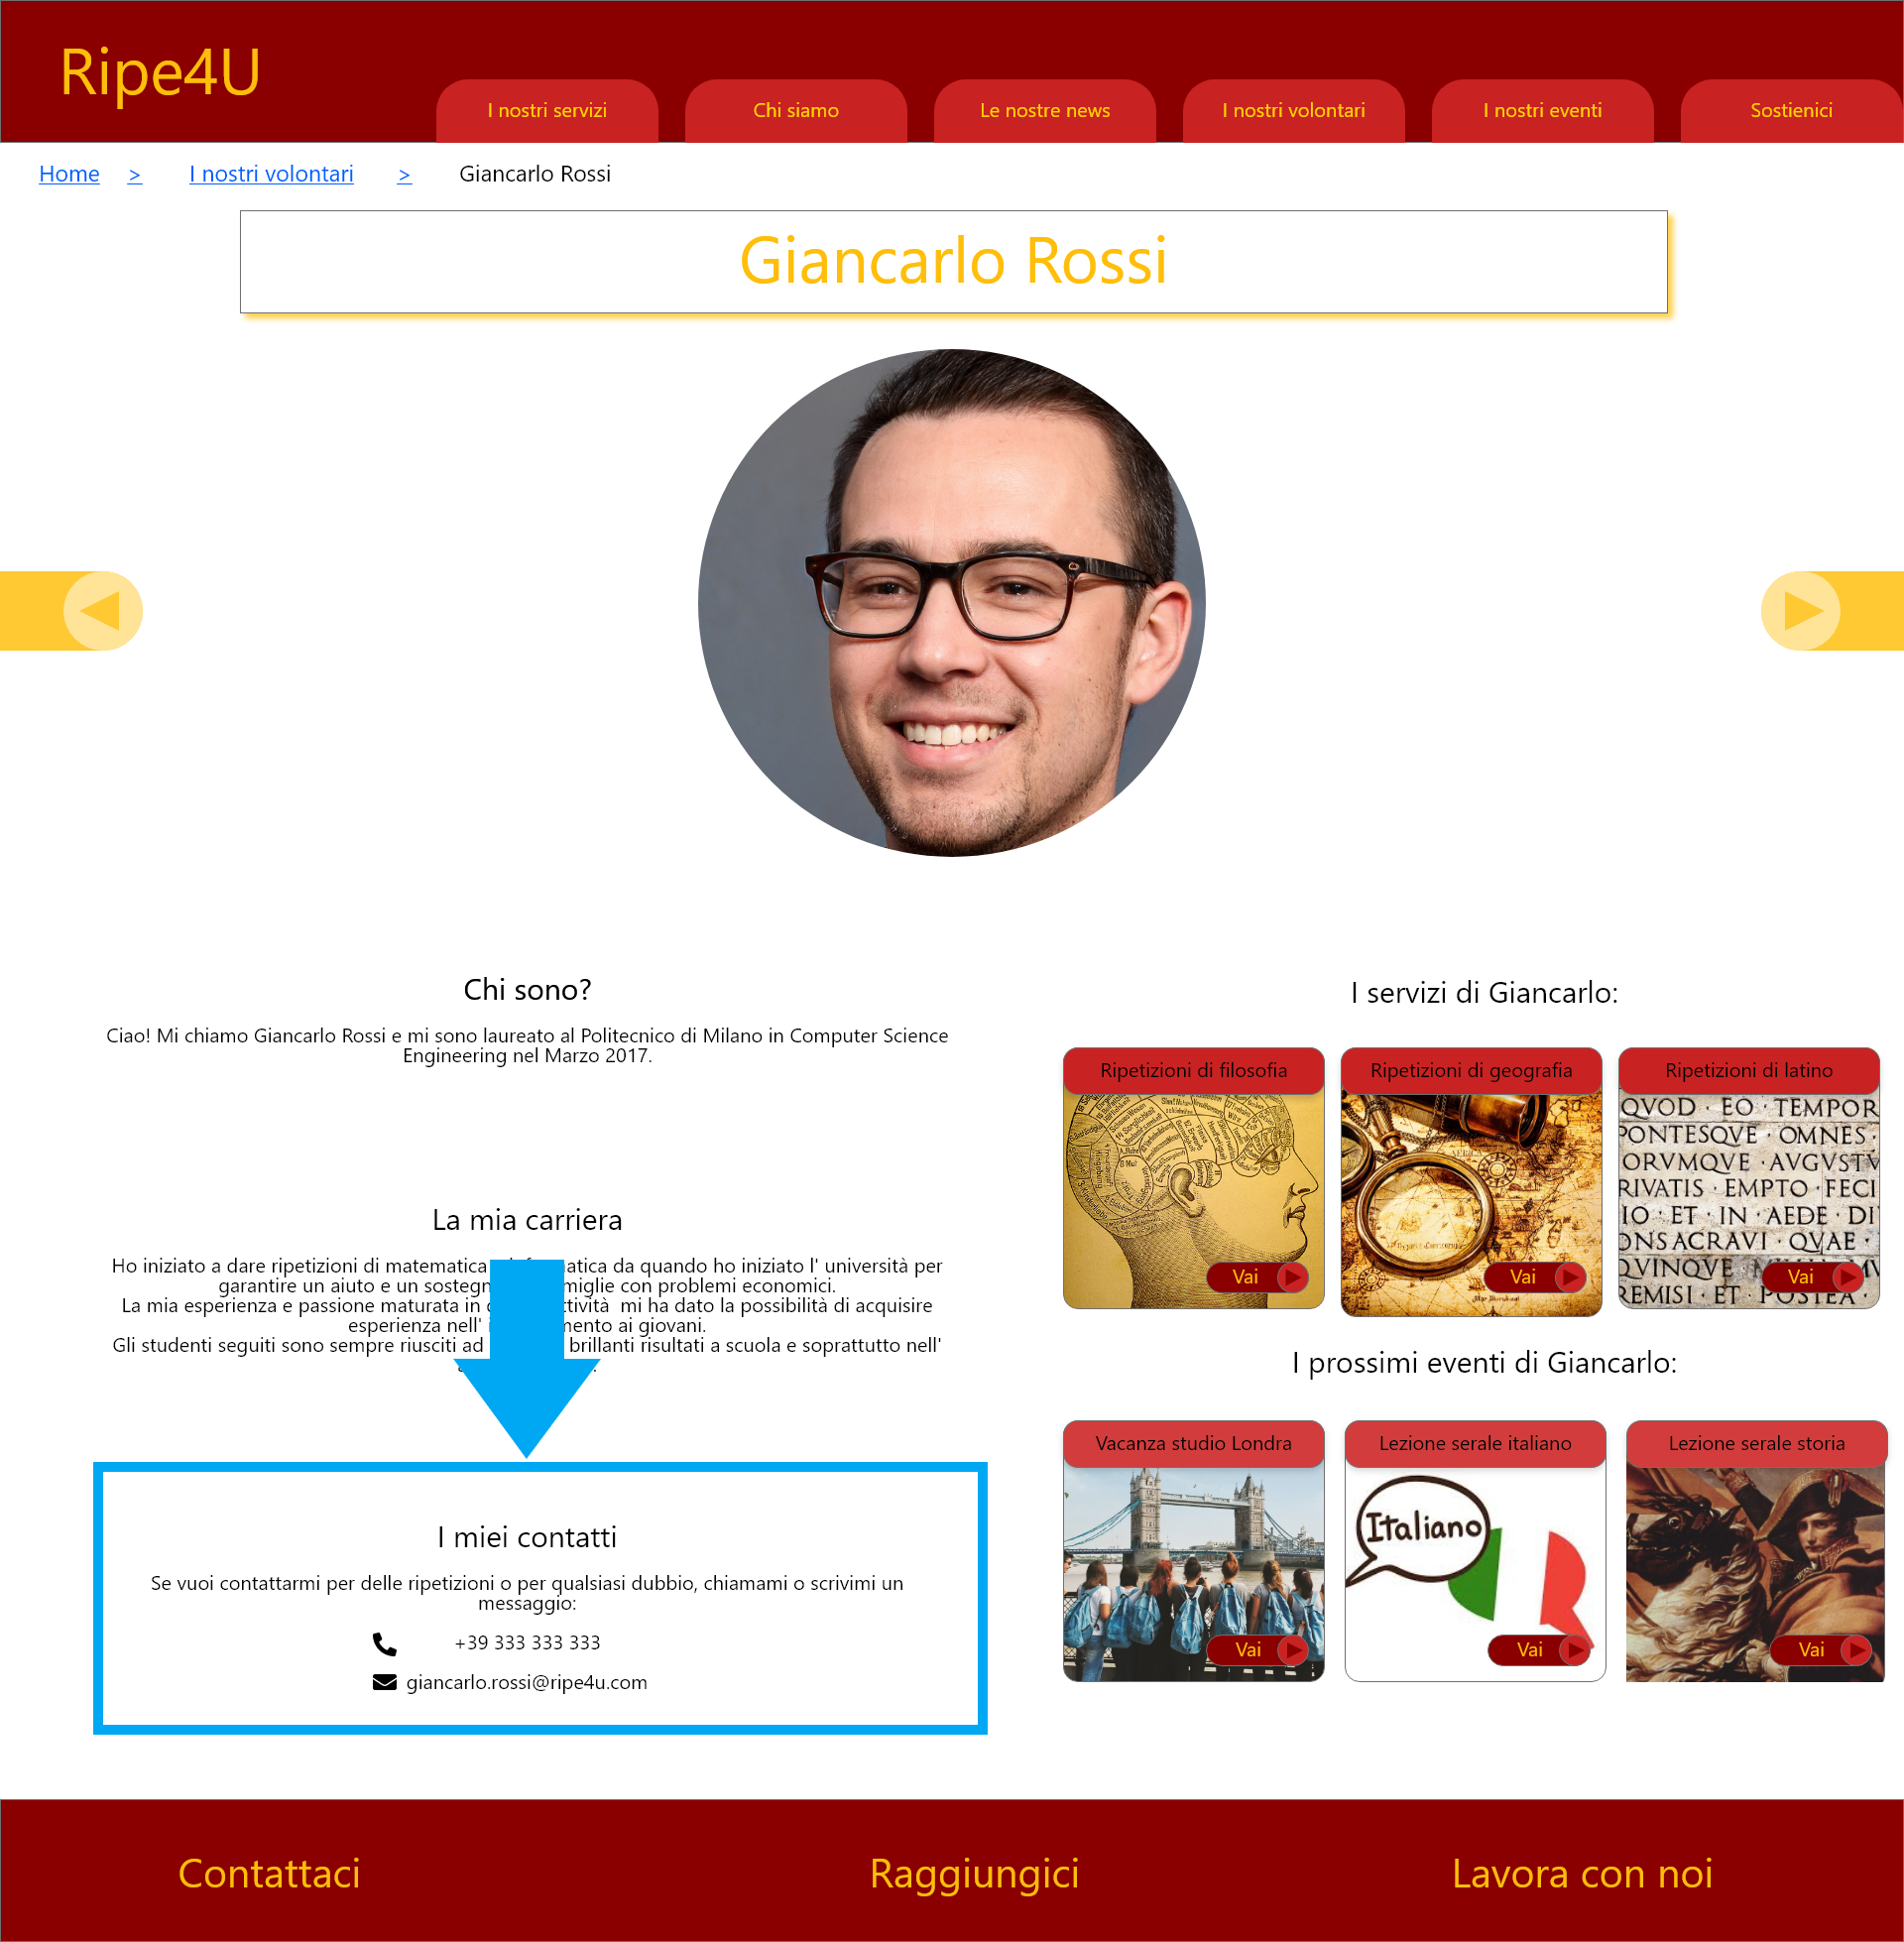
\includegraphics[scale=0.25]{resources/images/scenario1-5.png}
        \caption{I genitori possono vedere i contatti di Giancarlo Rossi}
    \end{figure}

    \newpage
    \section{Scenario 2}
    Luigi è uno studente universitario che vuole migliorare il proprio inglese
    per conseguire la certificazione richiesta e iscriversi al corso di laurea
    specialistica di Ingegneria al Politecnico. Lo studente decide quindi di cercare
    se ci sono vacanze studio in Inghilterra che gli possano permettere di
    esercitarsi nella lingua. Luigi accede alla home di Ripe4U e clicca su "I nostri
    Eventi" per accedere alla pagina con il medesimo nome. Una volta sulla pagina lo
    studente clicca sul menù a tendina "tutti gli eventi" e sceglie la voce
    vacanze studio, il sito carica quindi la pagina aggiornata con tutti gli
    eventi di quella categoria. In alternativa lo studente può
    verificare direttamente la presenza dell' evento scrivendo nella finestra
    "cerca" "vacanza studio a Londra". Luigi fa click sull' immagine con l'
    evento a cui è interessato per accedervi. La pagina caricata contiene tutte le
    informazioni principali sull' evento includendo il volontario organizzatore e un
    form dove inserire una mail per ricevere conferma della prenotazione del proprio
    posto.
    \begin{figure}[H]
        \centering
        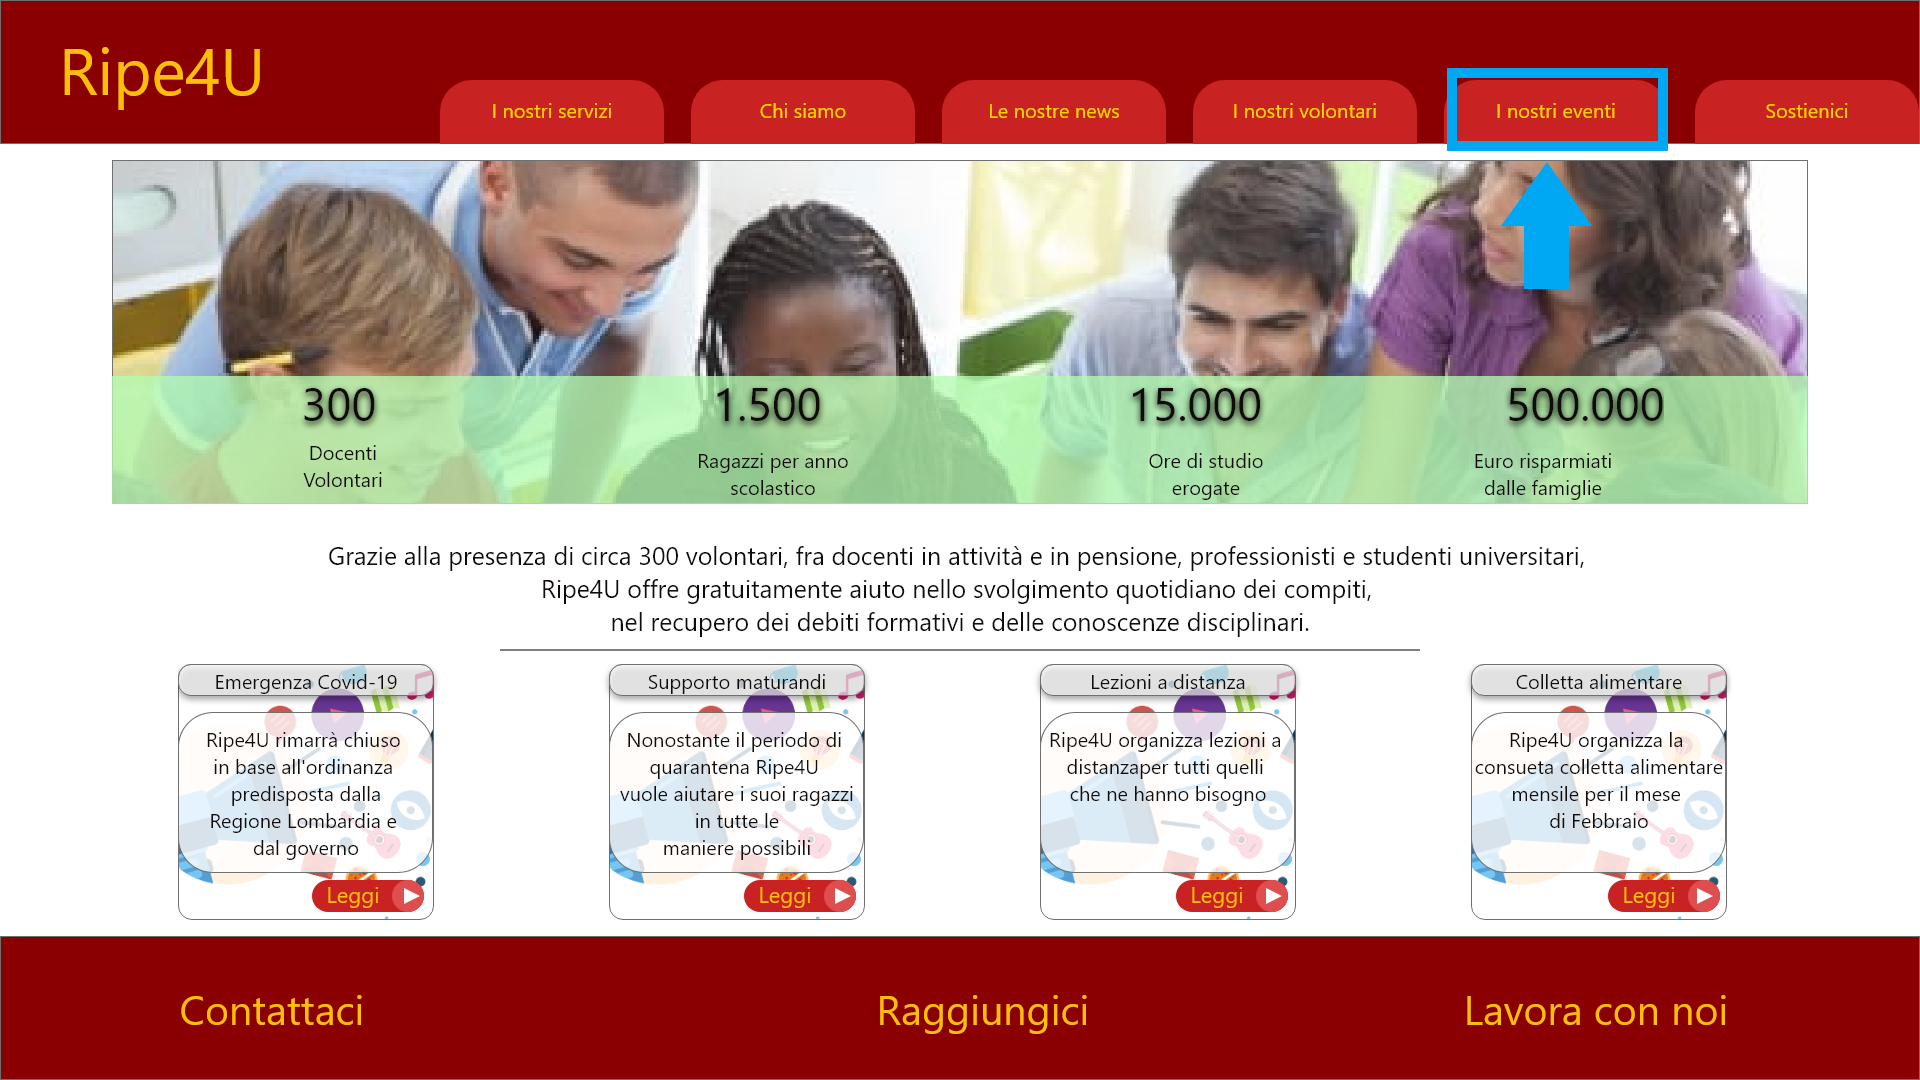
\includegraphics[scale=0.25]{resources/images/scenario2-1.png}
        \caption{Luigi clicca su "I nostri eventi"}
    \end{figure}
    \begin{figure}[H]
        \centering
        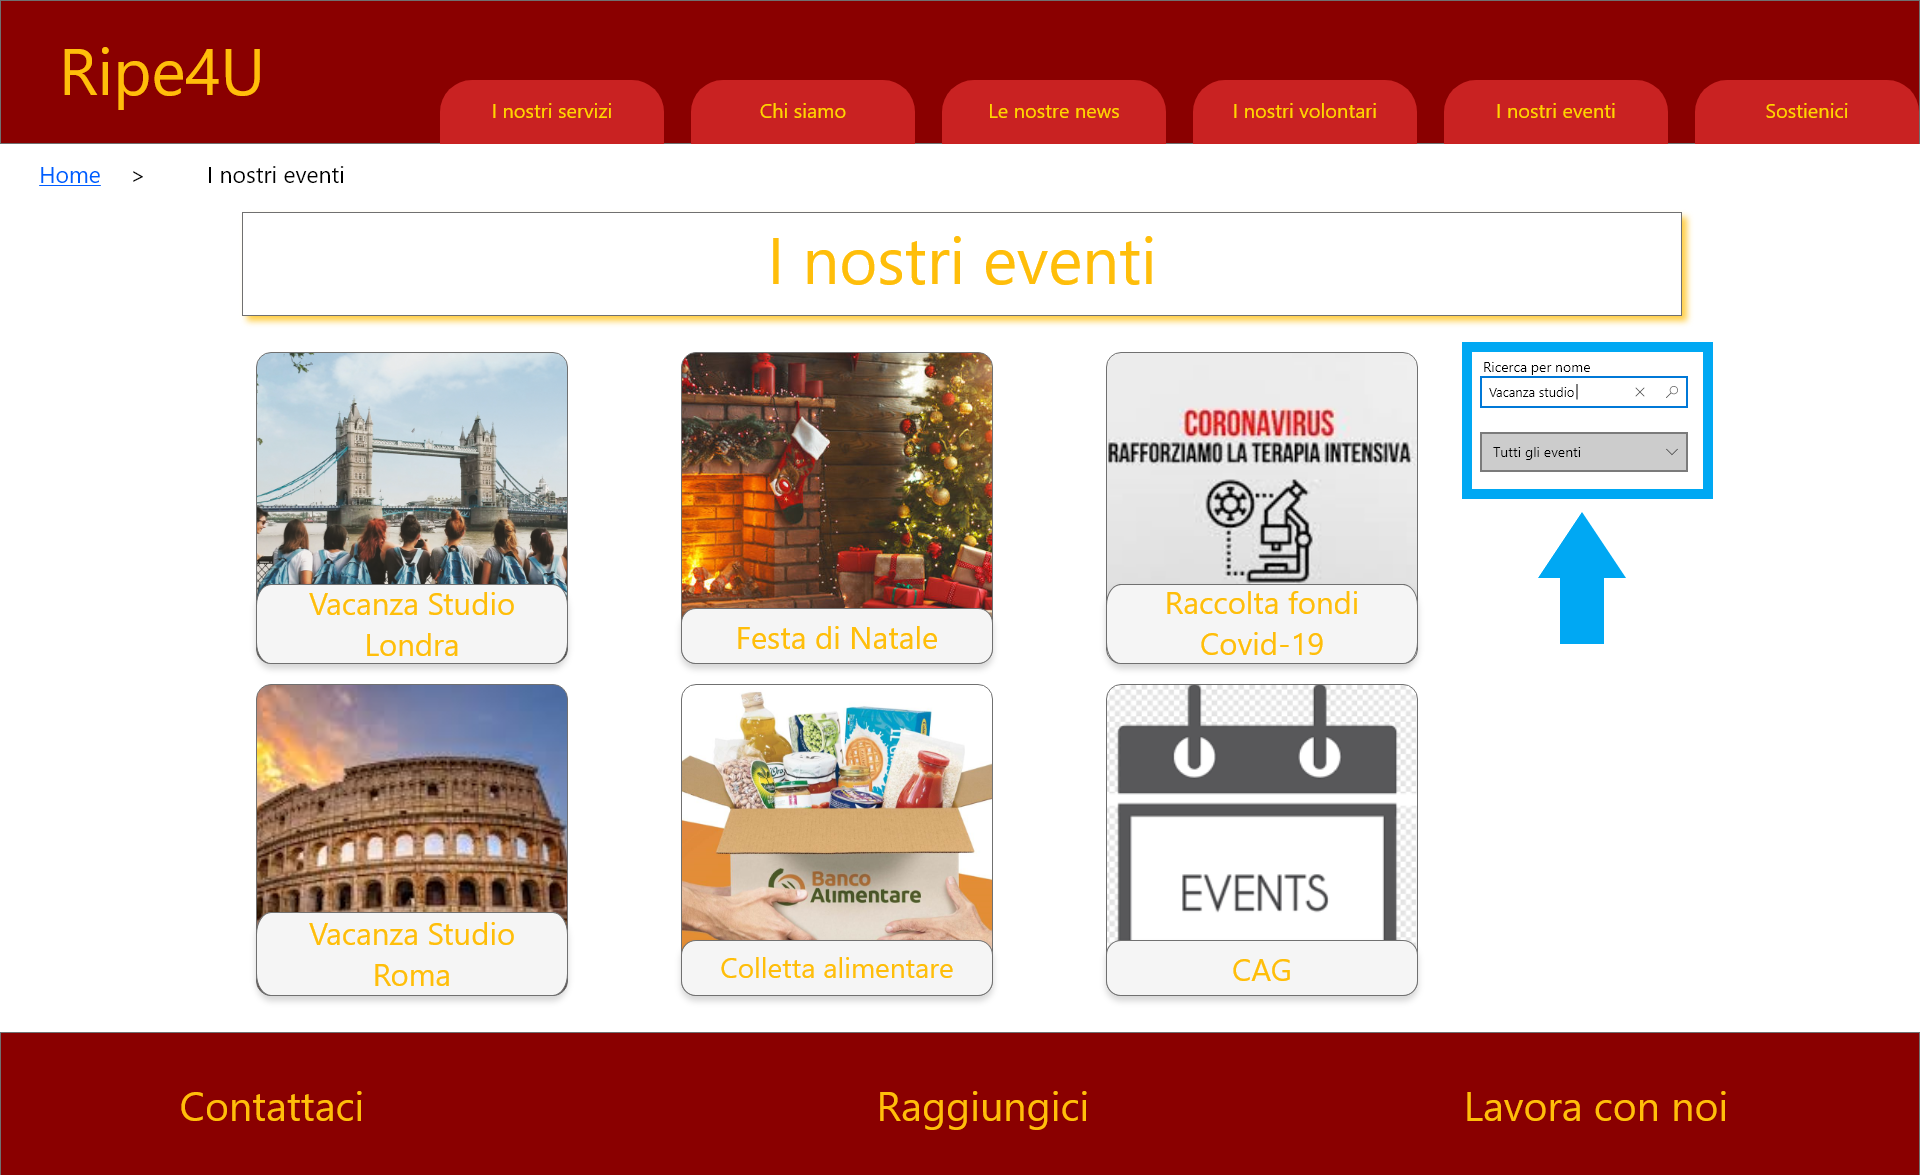
\includegraphics[scale=0.25]{resources/images/scenario2-2.png}
        \caption{Luigi cerca la vacanza studio}
    \end{figure}
    \begin{figure}[H]
        \centering
        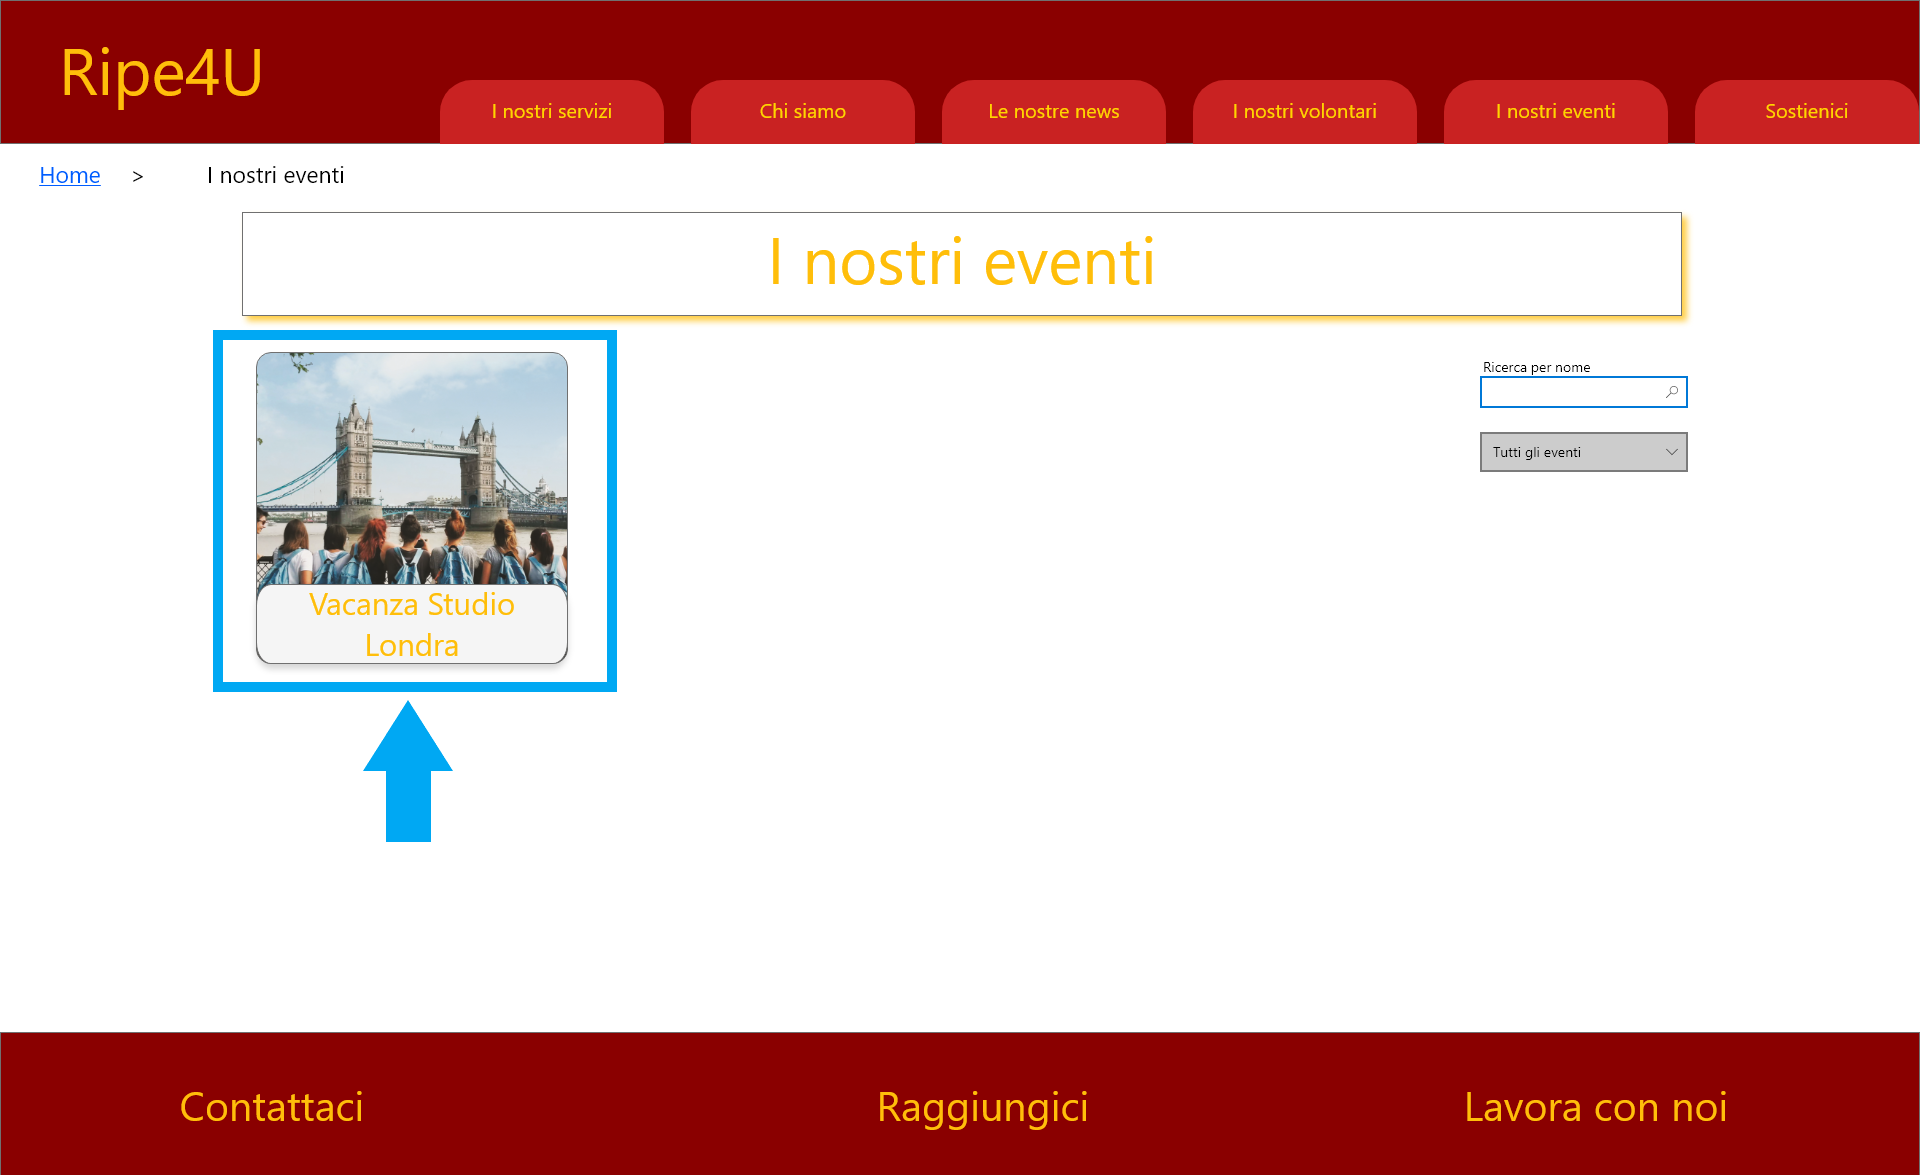
\includegraphics[scale=0.25]{resources/images/scenario2-3.png}
        \caption{Luigi clicca su "Vacanza Studio Londra"}
    \end{figure}
    \begin{figure}[H]
        \centering
        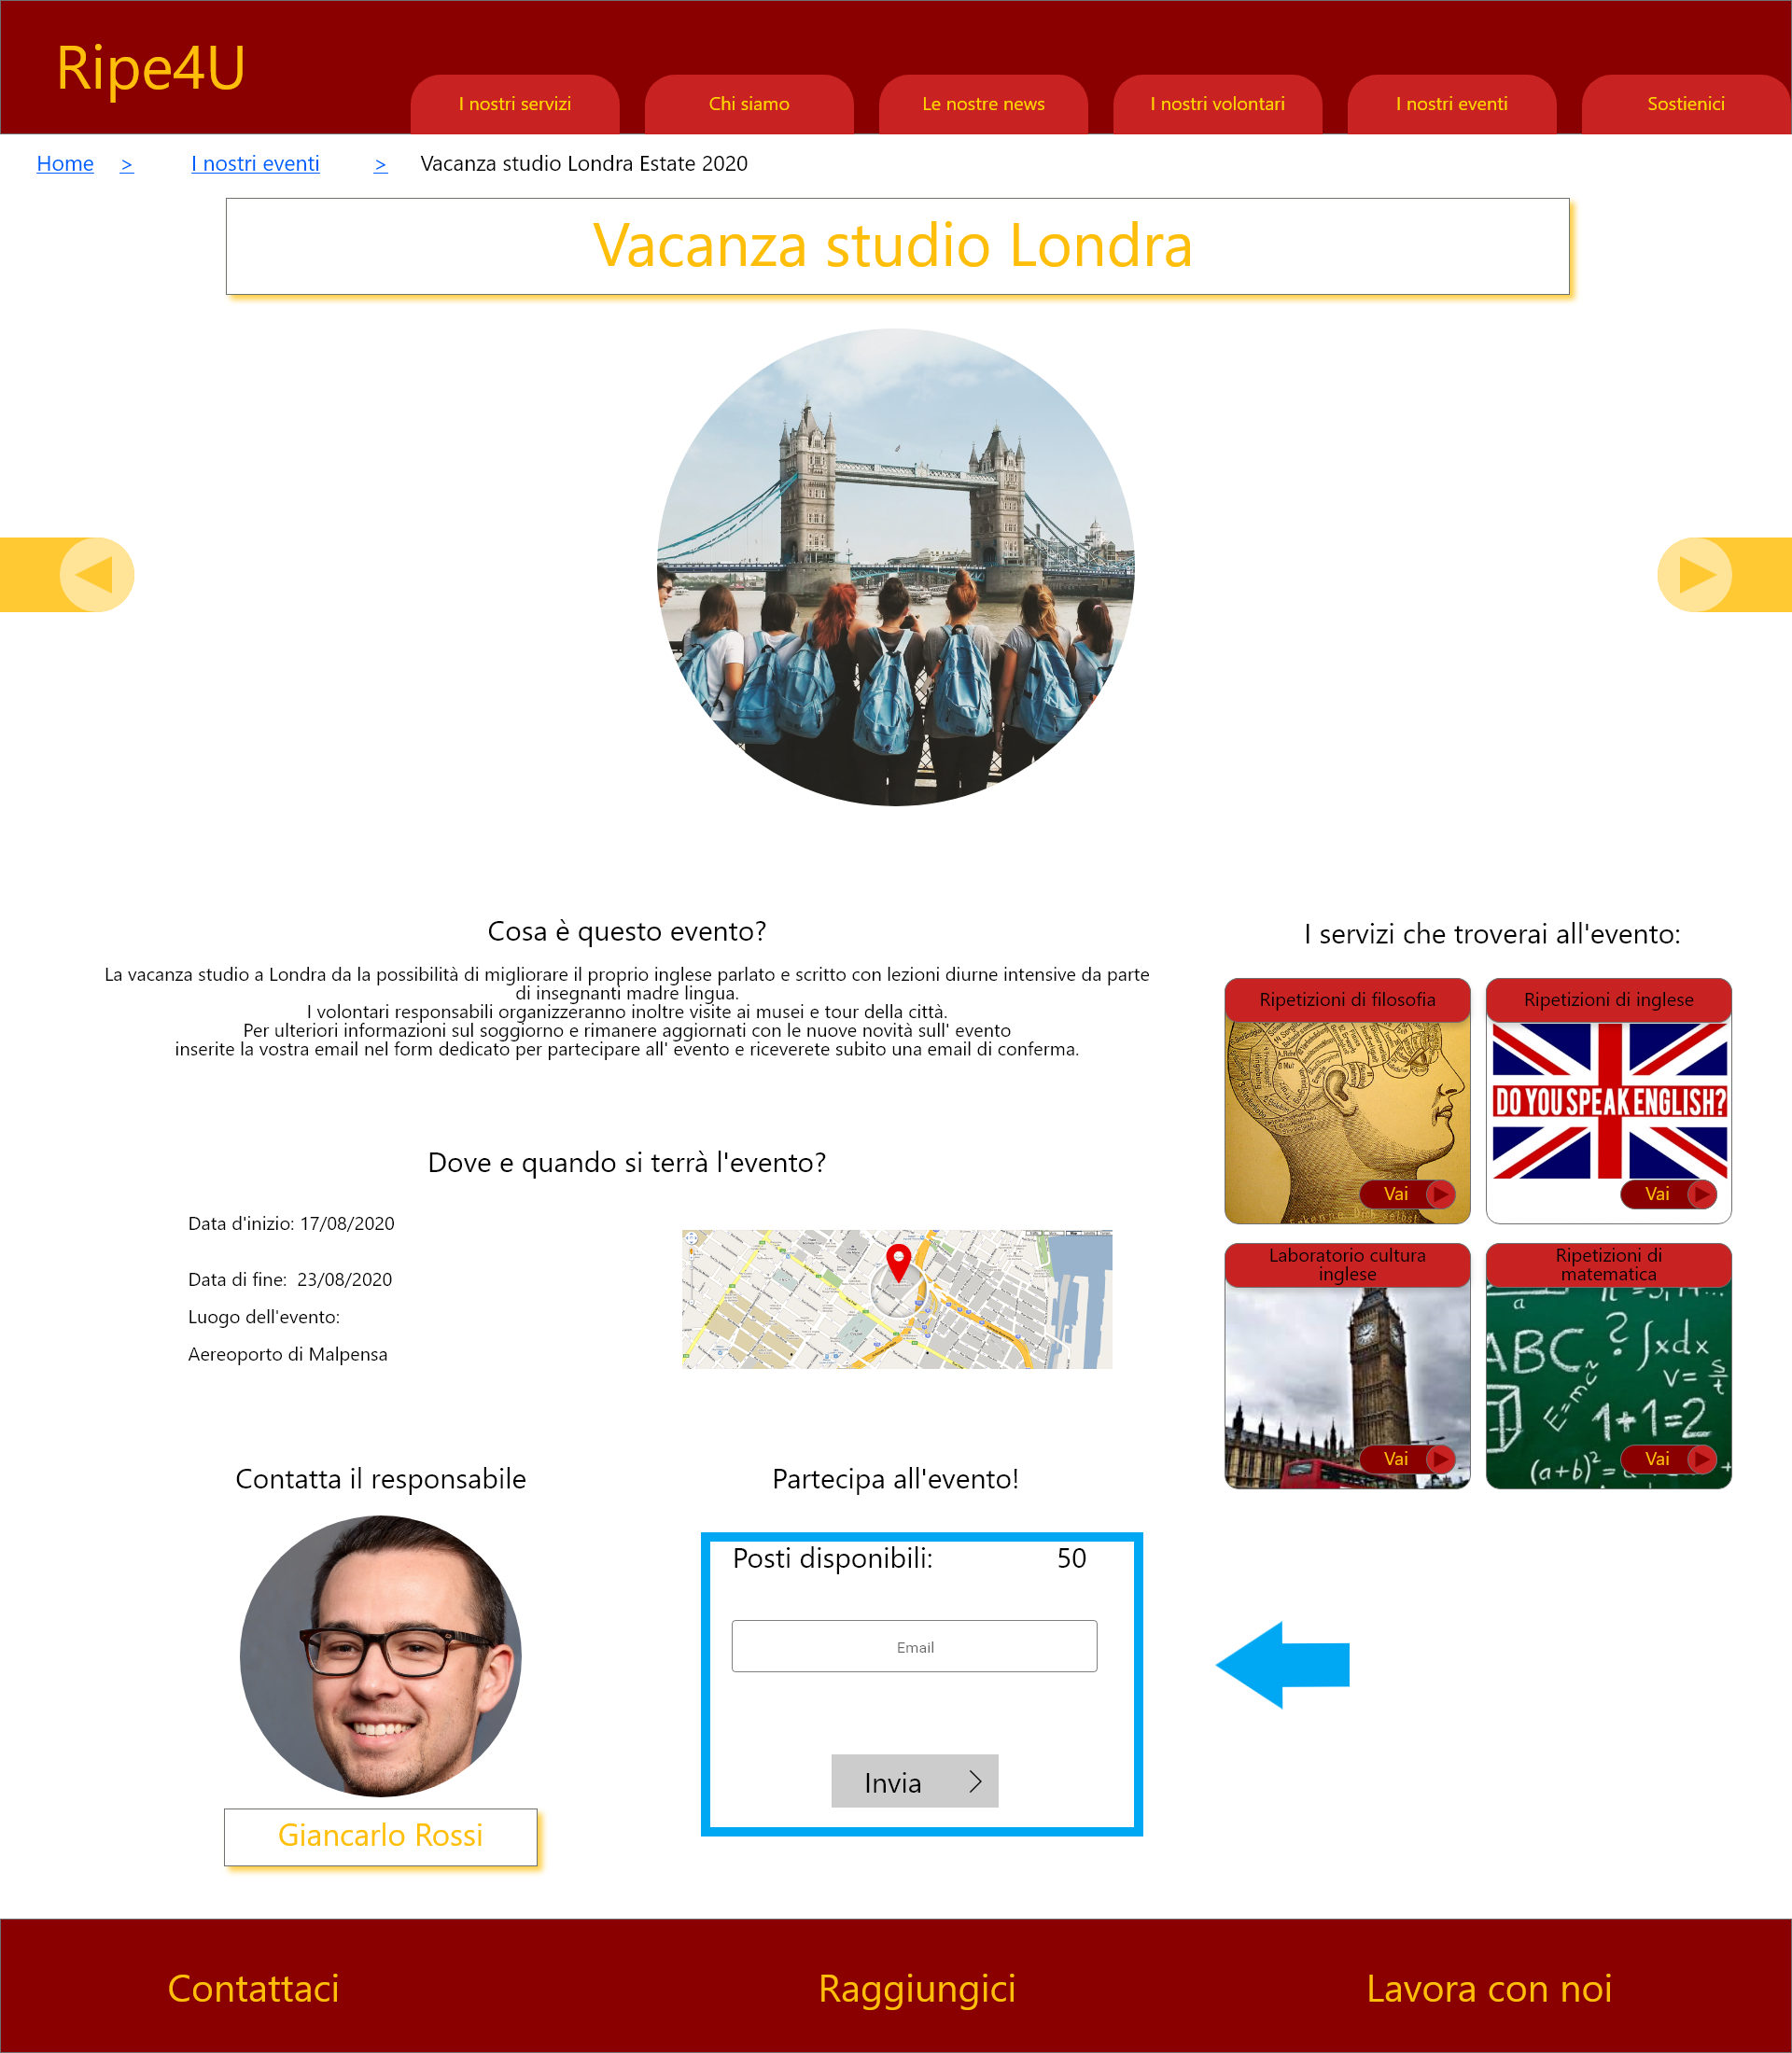
\includegraphics[scale=0.25]{resources/images/scenario2-4.png}
        \caption{Luigi inserisce la sua mail nel form per prenotarsi}
    \end{figure}
    \newpage
    \section{Scenario 3}
    Uno studente di nome Giuseppe, grazie alle ripetizioni di un professore
    volontario, si è sentito molto più sereno nello svolgere la versione di
    latino e per questo ha deciso di riorganizzare un incontro sempre con lo
    stesso volontario, ma non ricorda il suo contatto. Lo studente accede quindi
    alla Home di Ripe4U e clicca su "I nostri volontari". Il sito carica la
    pagina contenente le fotografie e i nominativi dei volontari. Lo studente
    scrive in "cerca" il nome del professore con cui vuole fare la ripetizione e
    una volta fatto invio sulla barra di ricerca, la pagina carica l'
    immagine profilo del professore. Lo studente cliccando sull' immagine
    accede alla pagina dettaglio del professore e può vedere, oltre a una breve
    descrizione e alla carriera, anche il contatto che cercava.
    \begin{figure}[H]
        \centering
        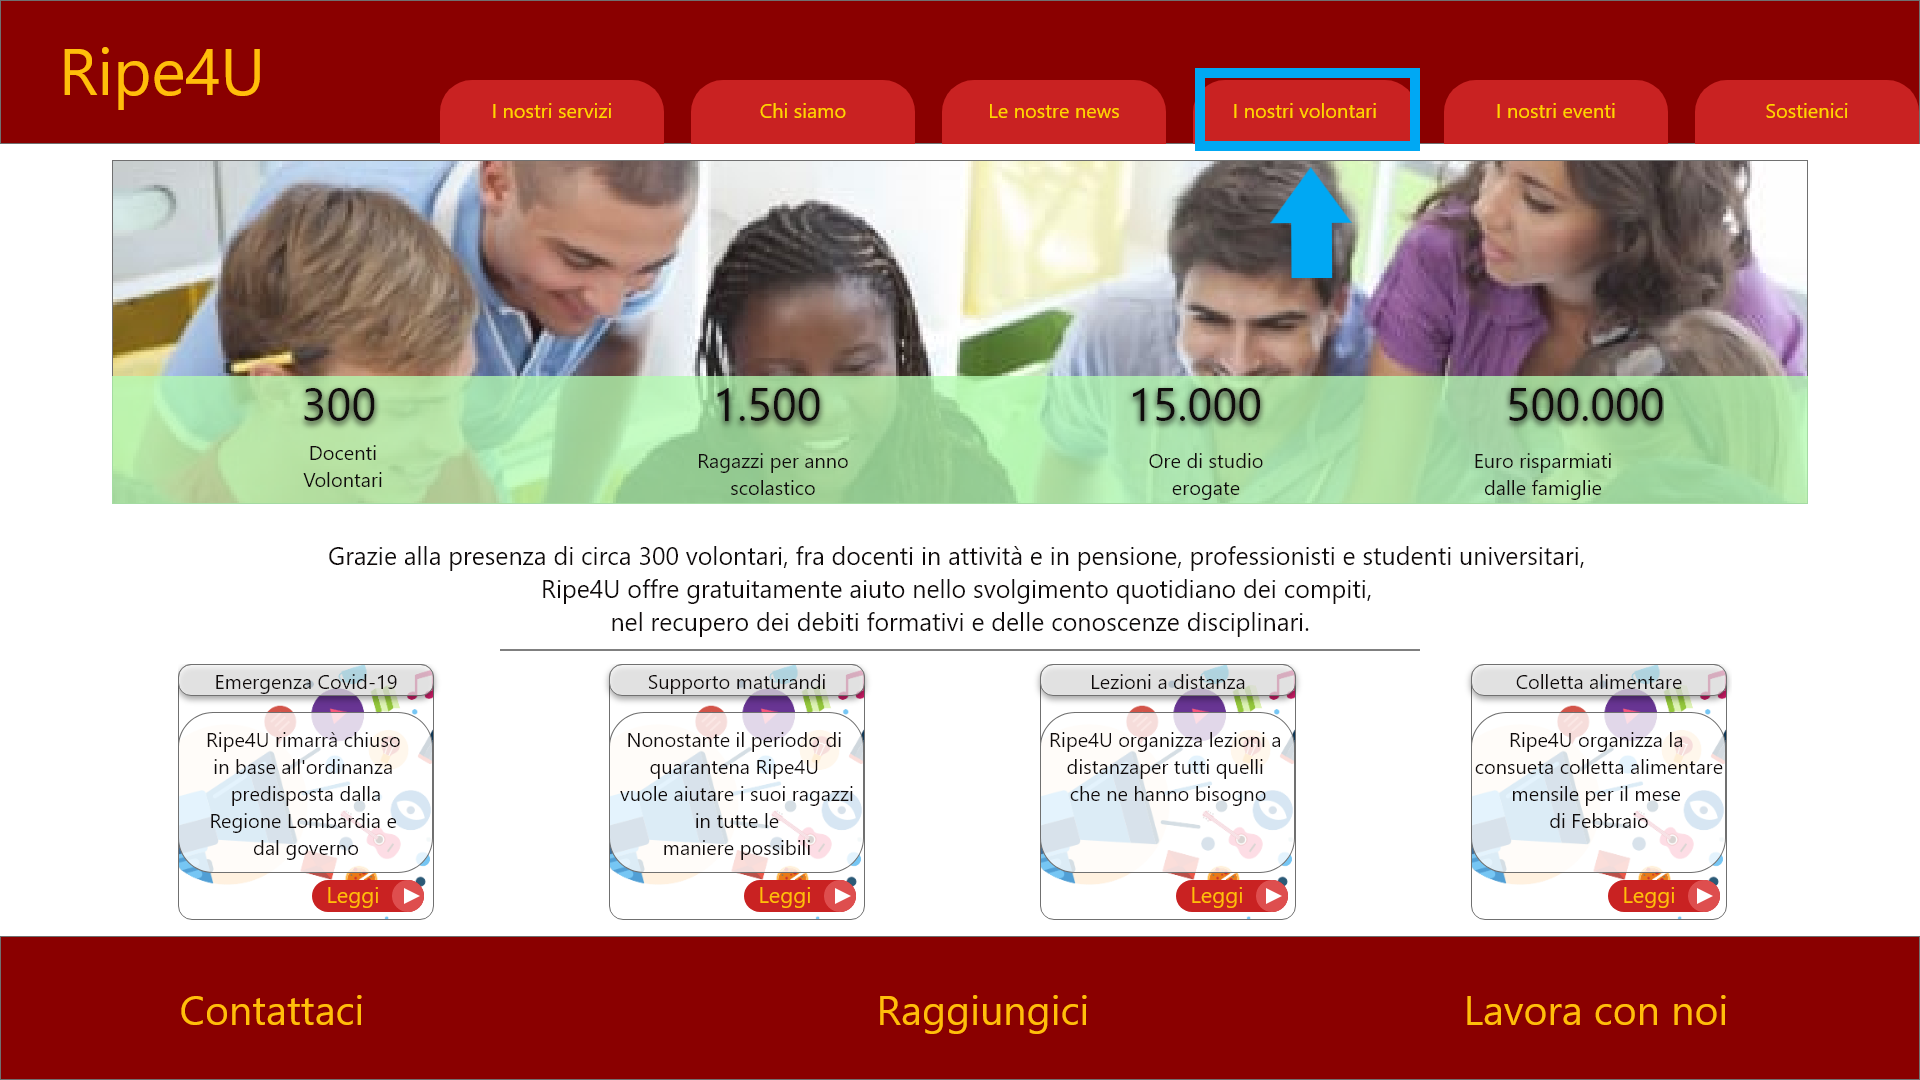
\includegraphics[scale=0.25]{resources/images/scenario3-1.png}
        \caption{Giuseppe clicca su "I nostri volontari"}
    \end{figure}
    \begin{figure}[H]
        \centering
        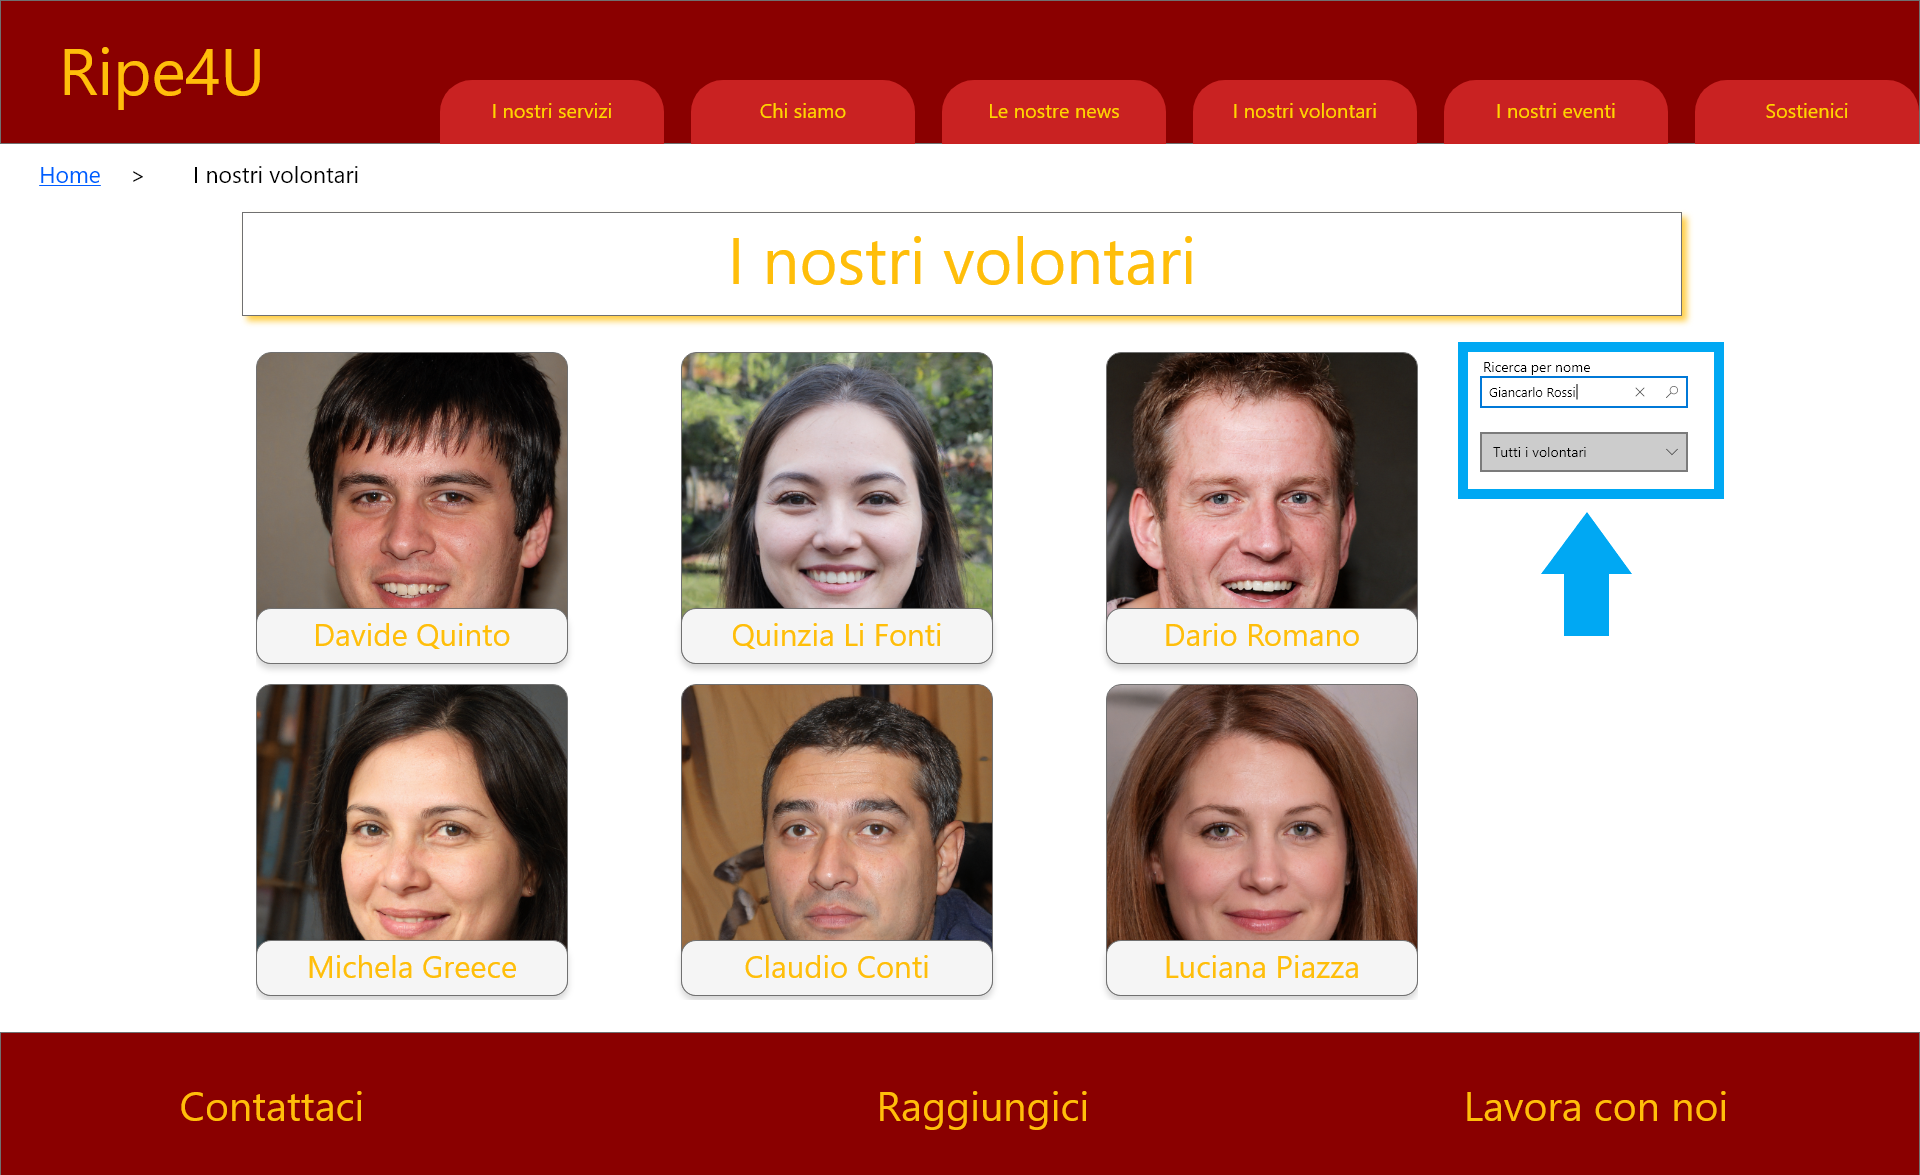
\includegraphics[scale=0.25]{resources/images/scenario3-2.png}
        \caption{Giuseppe cerca "Giancarlo Rossi"}
    \end{figure}
    \begin{figure}[H]
        \centering
        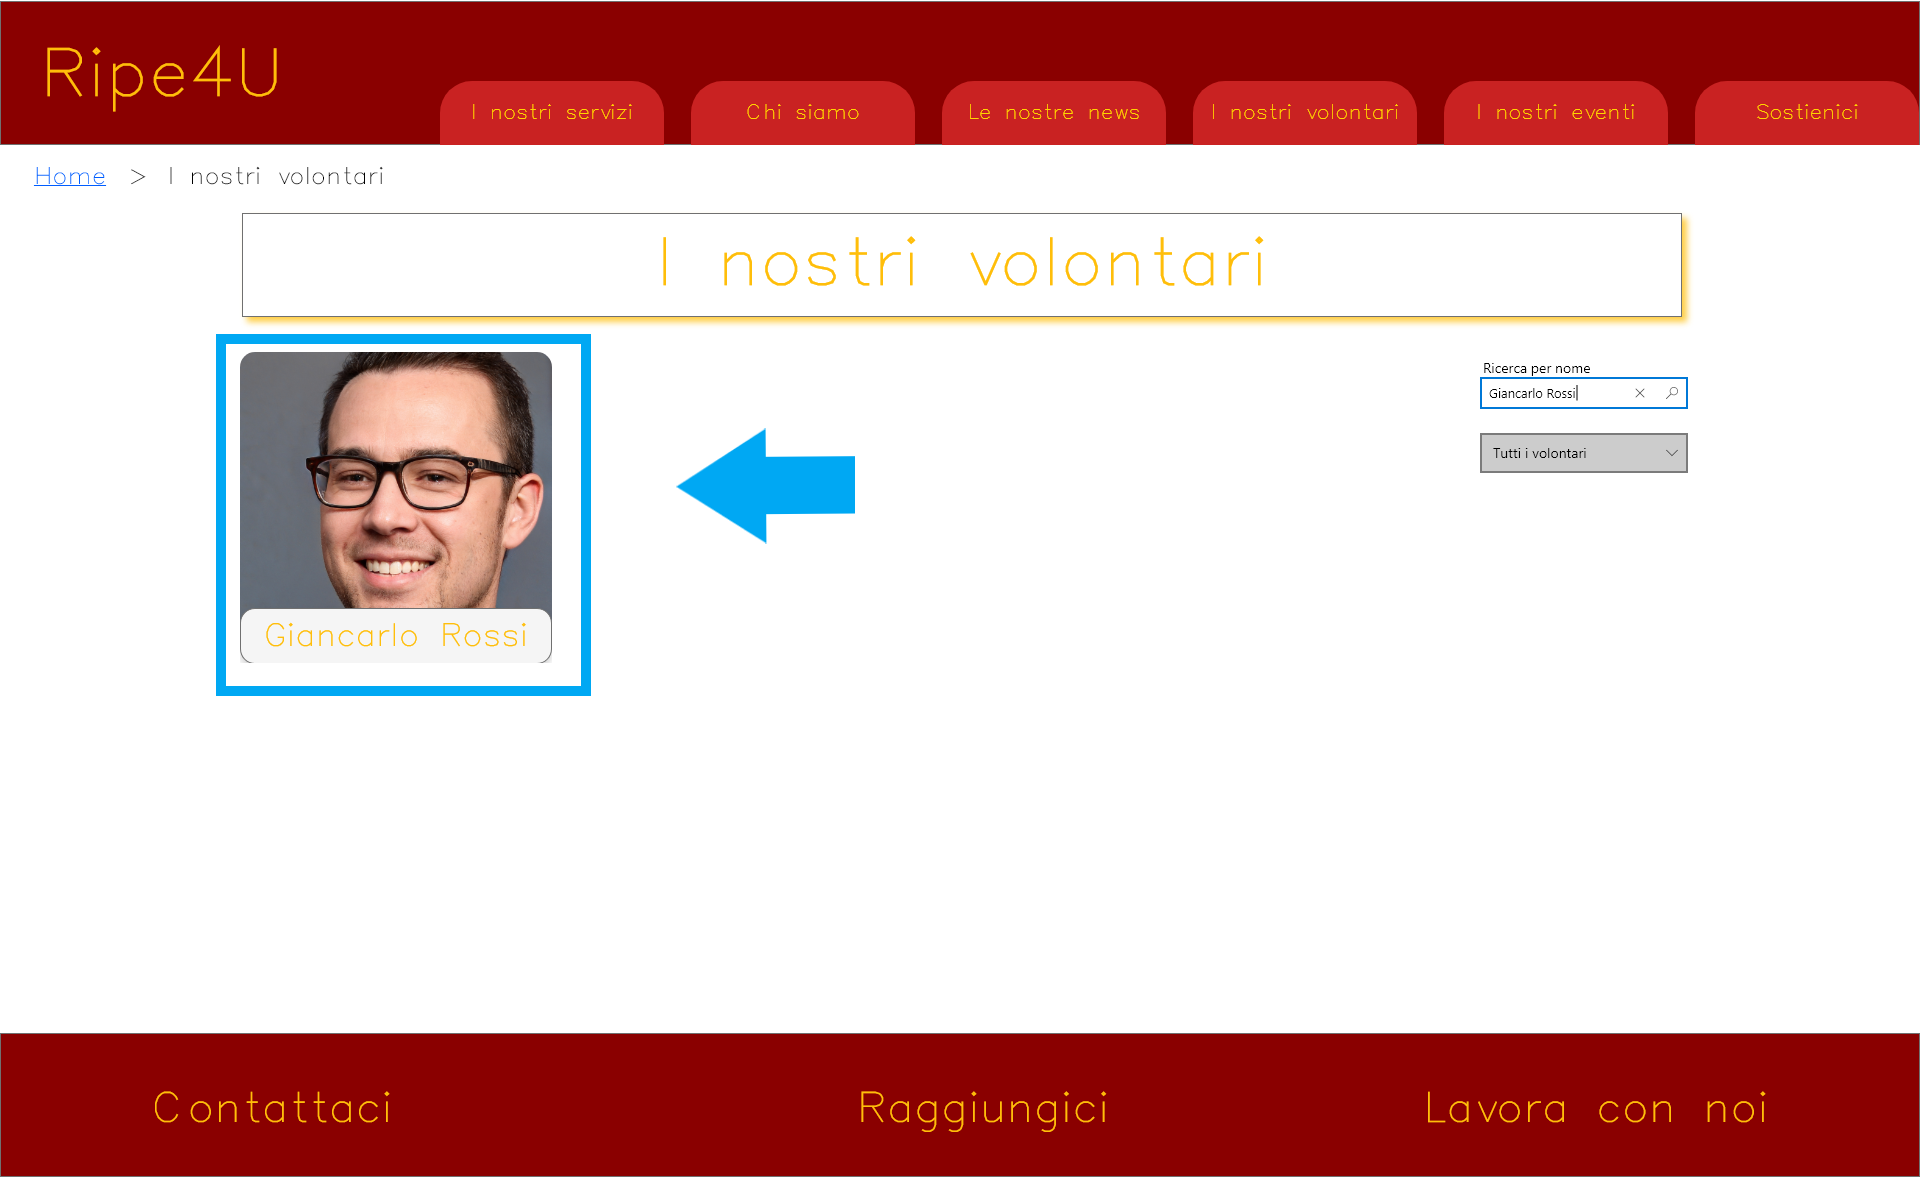
\includegraphics[scale=0.25]{resources/images/scenario3-3.png}
        \caption{Giuseppe clicca su "Giancarlo Rossi"}
    \end{figure}
    \begin{figure}[H]
        \centering
        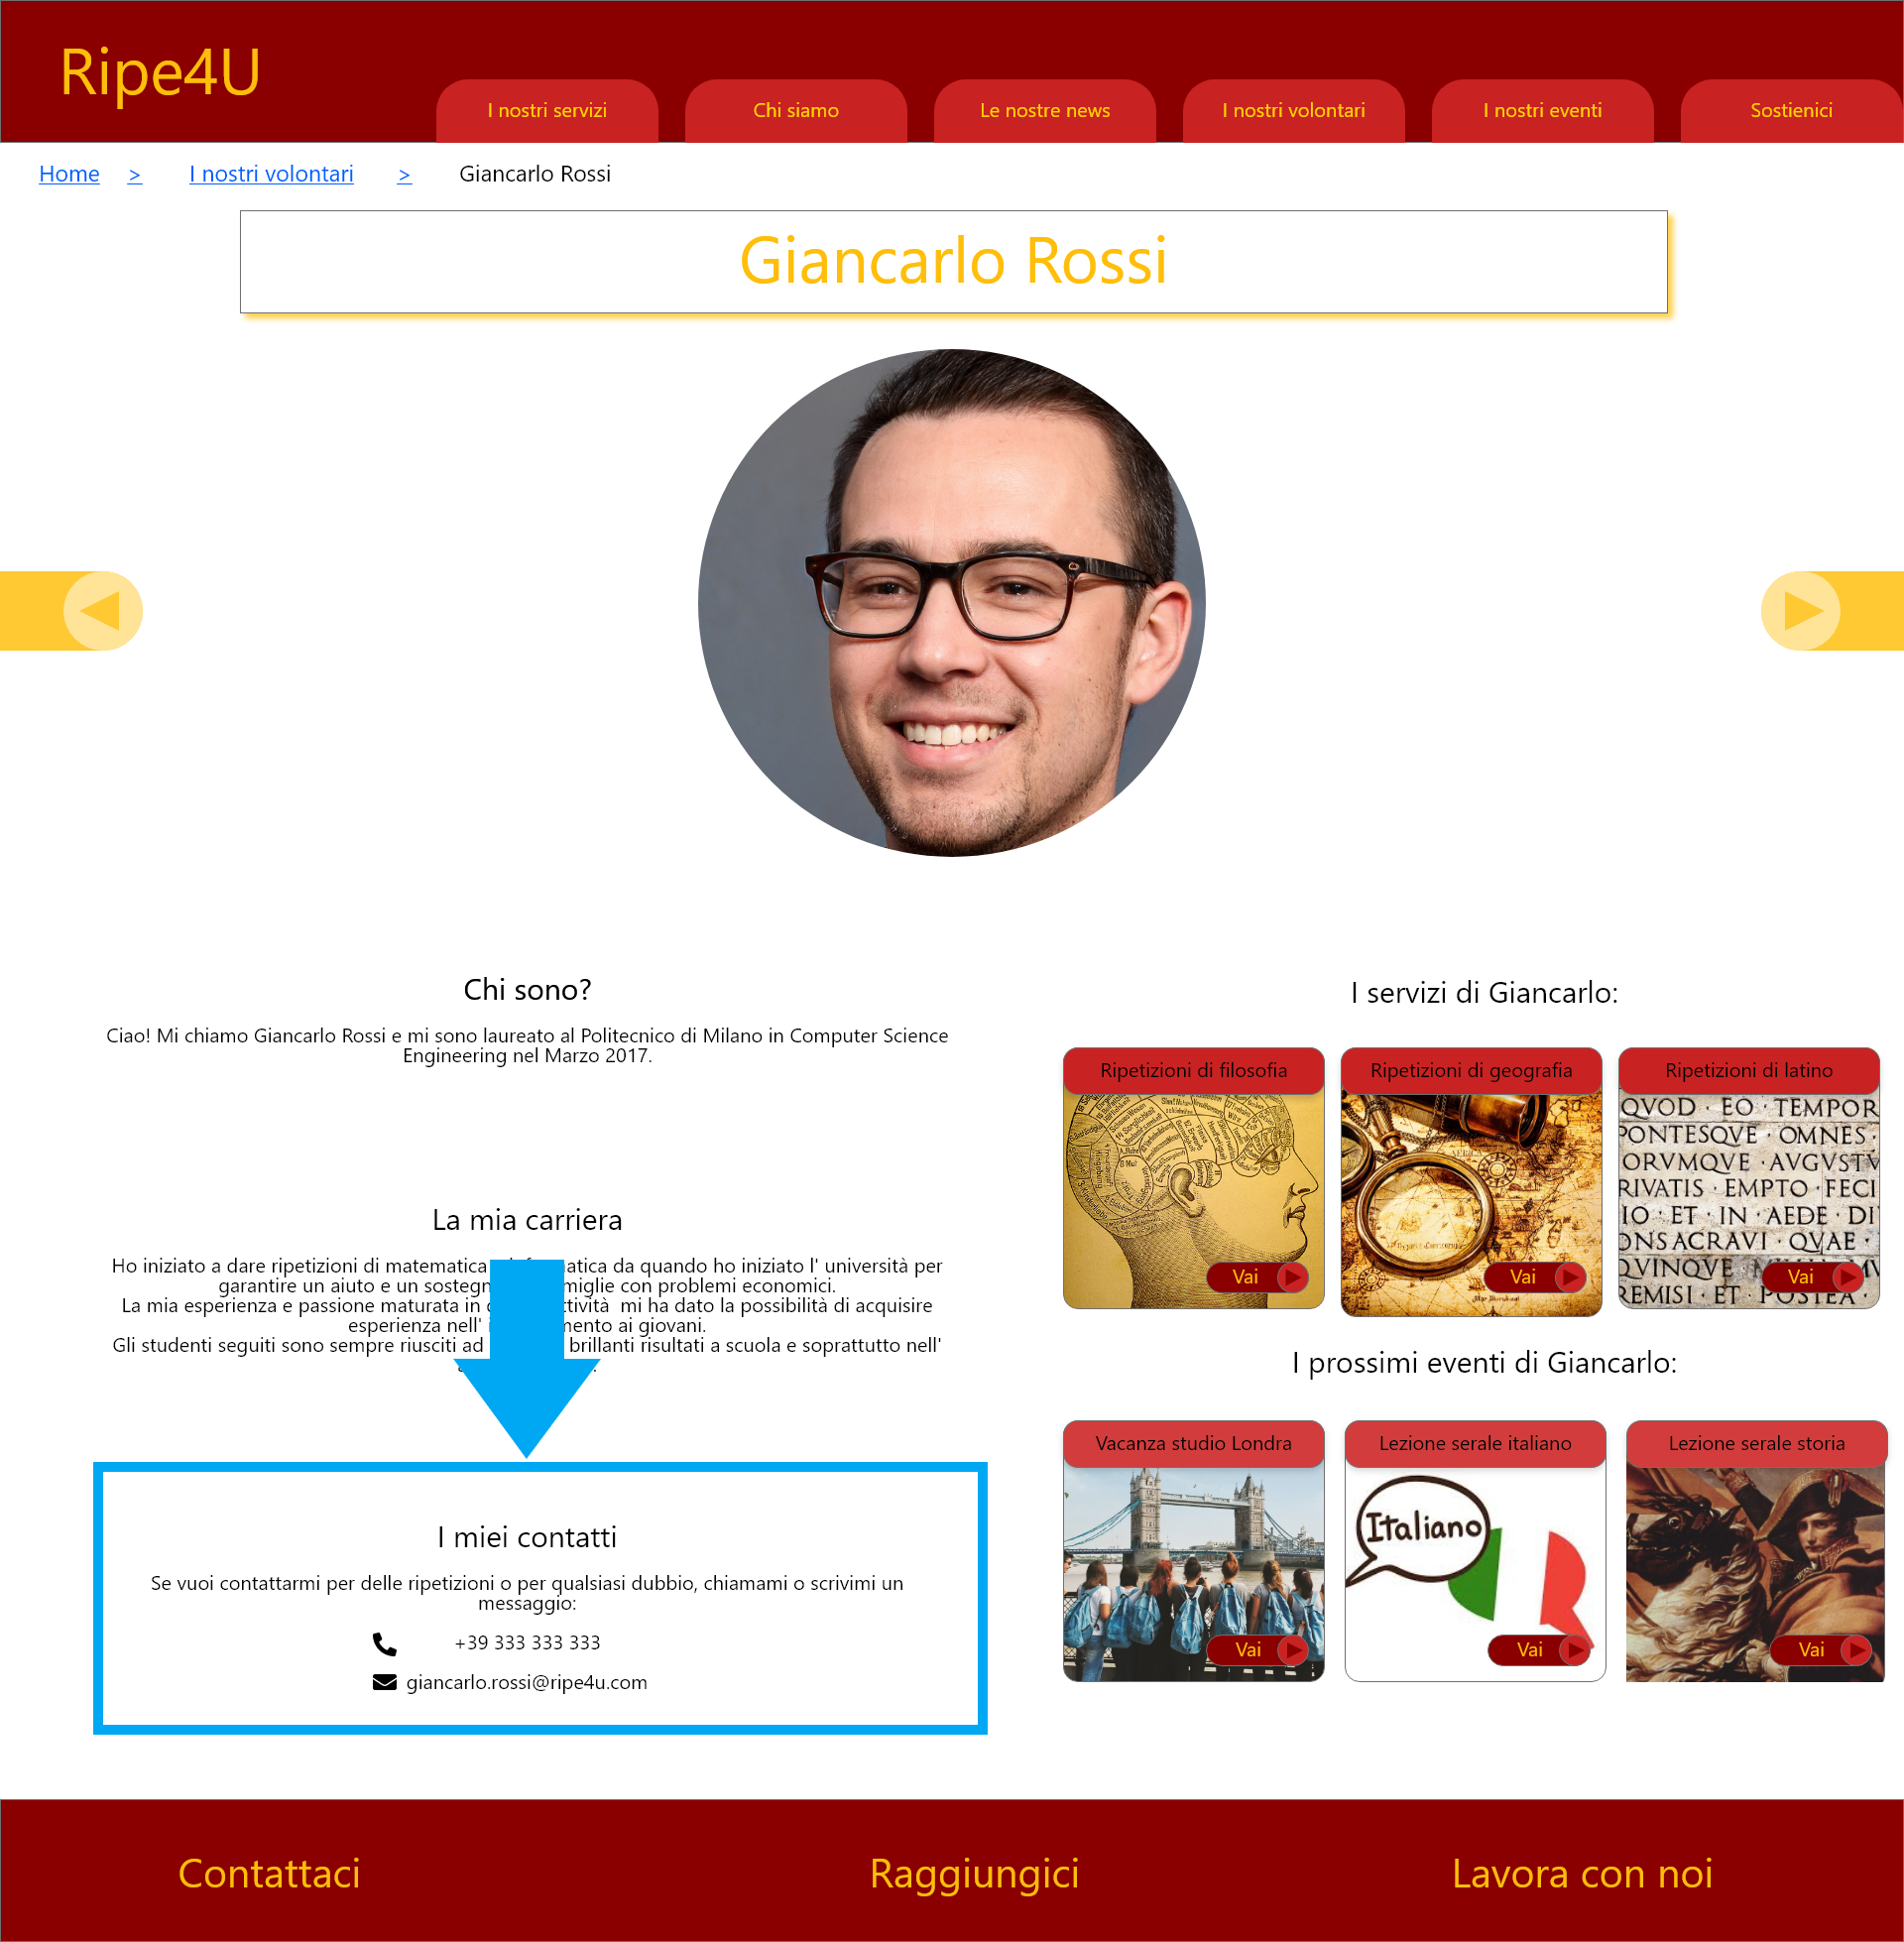
\includegraphics[scale=0.25]{resources/images/scenario3-4.png}
        \caption{Giuseppe ha trovato i contatti di Giancarlo Rossi}
    \end{figure}
 